% !TeX root = ../main.tex
% Add the above to each chapter to make compiling the PDF easier in some editors.

\chapter{Experiments}

% \gls{wa} framework: what? where? (Part I) feedthrough (Part II) anicipation and coordination of actions (Part III) <==== i.e. this goes at the description of the final study
% Note also that the sound is rendered with respect to the spatial position and orientation of the head-mounted display.

In total, five experiments were conducted for this thesis. Two were quick proof-of-concept experiments to validate the initial speculation, two - pilot studies to determine values for some properties of the final experiment and test the process of sampling participants on \gls{wa} index, and one formal study to test \nameref{final_study}. 
In all the experiments participants were alone in the \gls{ve}.

\paragraph{Apparatus} % and design}
Relatively similar apparatus was used across all studies:
experiments were implemented with the help of Unity3d  2018.1.5f1; audio spatialisation tool was Resonance Audio SDK for Unity, version 1.2.1 with sound occlusion turned off; hardware-wise, HTC Vive \gls{vr} and Oculus Rift headsets, 6 \gls{dof} controllers, along with on-ear stereo headphones, and a Windows 10 PC. 

%The design of all the experiments was similar in regard to how they approached collaboration: all the studies were a simulation of collaborative use case, meaning that 

\section{Proof of Problem}

Initial motivation for this work was a question of whether sudden events (movements of the buildings) in \gls{vr} would cause uncomfortable experience for users (Fig. \ref{fig:a1unawareofa2actions}). Two prototypes were developed to validate this motivation, these are described in the \nameref{par:appearing_building} and \nameref{par:approaching_building} paragraphs.

\begin{figure}
	\centering
	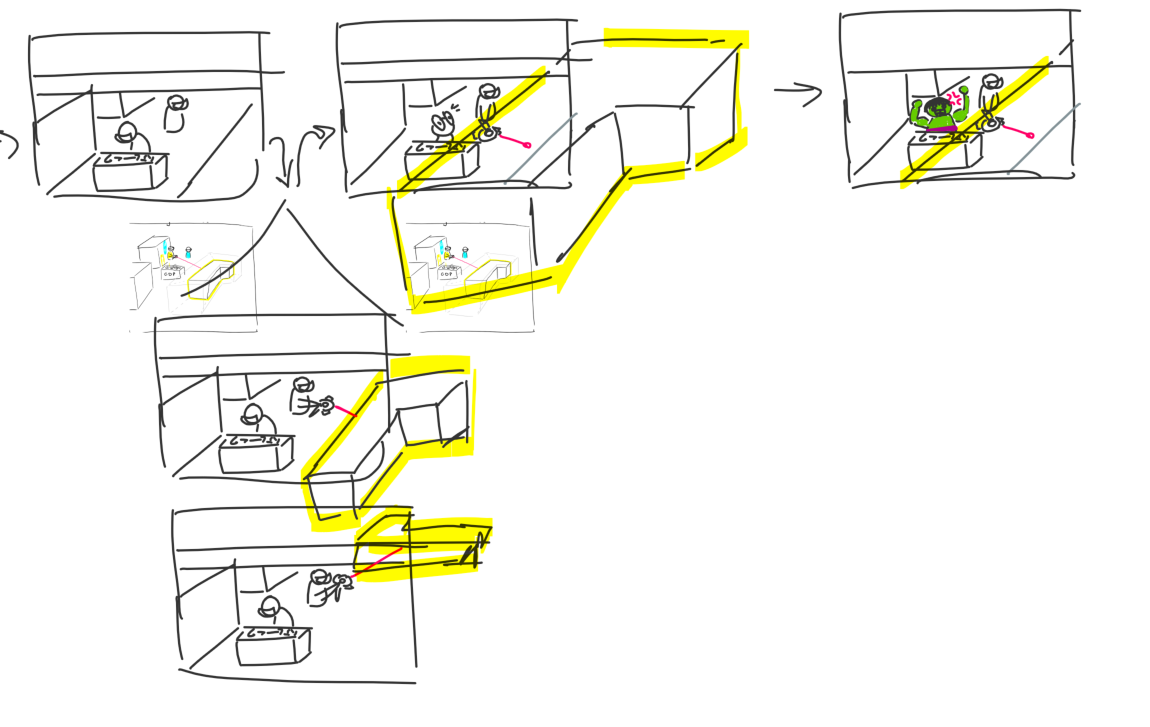
\includegraphics[width=0.7\linewidth]{figures/placeholders/A1_unaware_of_A2_actions}
	\caption{Collaborators unaware of each other's actions}
	\label{fig:a1unawareofa2actions}
\end{figure}

\paragraph{Appearing building} 
\label{par:appearing_building}
The first prototype looked into how the participants' experience would be influenced, if a building suddenly appeared in-front of them, when they were occupied with their own task.

% Participants
Three participants (all male) were chosen among the members of the \gls{hci} group at the University of Otago. Two had prior experience in \gls{vr}, one had not.

% Procedure & Task
Participants were placed in the immersive \gls{vr} environment, which constituted of 3D approximations of buildings at the campus of the University of Otago and surrounding districts. First, the the affordances of the environment were introduced: teleportation, walking and looking around; then participants were asked to navigate to the university clock tower. During this navigation task, a building would pop up in-front of them multiple times at experimenter's disposal. After the completion of the experiment the participants were asked to describe the experience, especially the parts, where a building appeared in-front of them.

% Apparatus (i.e Unity, Resonance Audio, stereo headphones, Vive)
%Unity3d and Oculus Rift \gls{hmd} with Touch Motion controllers were used in this experiment.

% Results
The participant with no prior experience in \gls{vr} described the experience as unexpected, but was also not sure, whether he caused it. The other two participants indicated that they were a bit stuttered by the experience, but in general, "didn't care much for it". Additionally, the participants described the experience as irritating, when the building continued to repeatedly appear after the first encounter.
% Limitations
% I do not check if anyone is concerned with the moving buildings when they get used to it.
% This doesn't matter tho, because according to the WA, people should know what the others are doing in the same environment.
% Discussion of the results?
%...

\paragraph{Approaching buildings}
\label{par:approaching_building}
In the second prototype the decision was made to move closer to the initial concern: buildings moving through and close to users in immersive \gls{vr} environment.
%Due to the results of the first experiment, the problem was regarded as worthwhile of further exploration. For the second proof of concept, a decision was made to come a bit closer to the initial motivation: buildings moving in \gls{ve}.

% Participants
4 new participant (all male) were chosen among the members of \gls{hci} group at the University of Otago; none of them took part in the previous experiment. Two had moderate and two had little experience with the \gls{vr} technology.

% Procedure & Task
The environment affordances of the environment remained the same, as in the previous prototype. The introduction remained the same, as well. The task was extended, so that when participants find the clock tower, they were asked to assume their place at the specially prepared viewing spot (Fig. \ref{fig:prototype2viewvingspot}). At this point the participants were asked to observe the clock tower and tell the experimenter, if anything seemed odd about its features (some elements of the tower were slightly off axis: see Fig. \ref{fig:prototype2clocktoweroddfeatures}). This was done to distract participants, and suddenly initiate the movement of the clock tower towards them. The speed of the clock tower building was 200 units (meters) per second, the initial distance from the viewing spot to the tower was approximately 69 meters; the clock tower would stop 0.5 meters in-front of a participant. At this point the experiment would finish, and the participants would be asked about their experience.

% TODO: indicate the viewing spot better
\begin{figure}
	\centering
	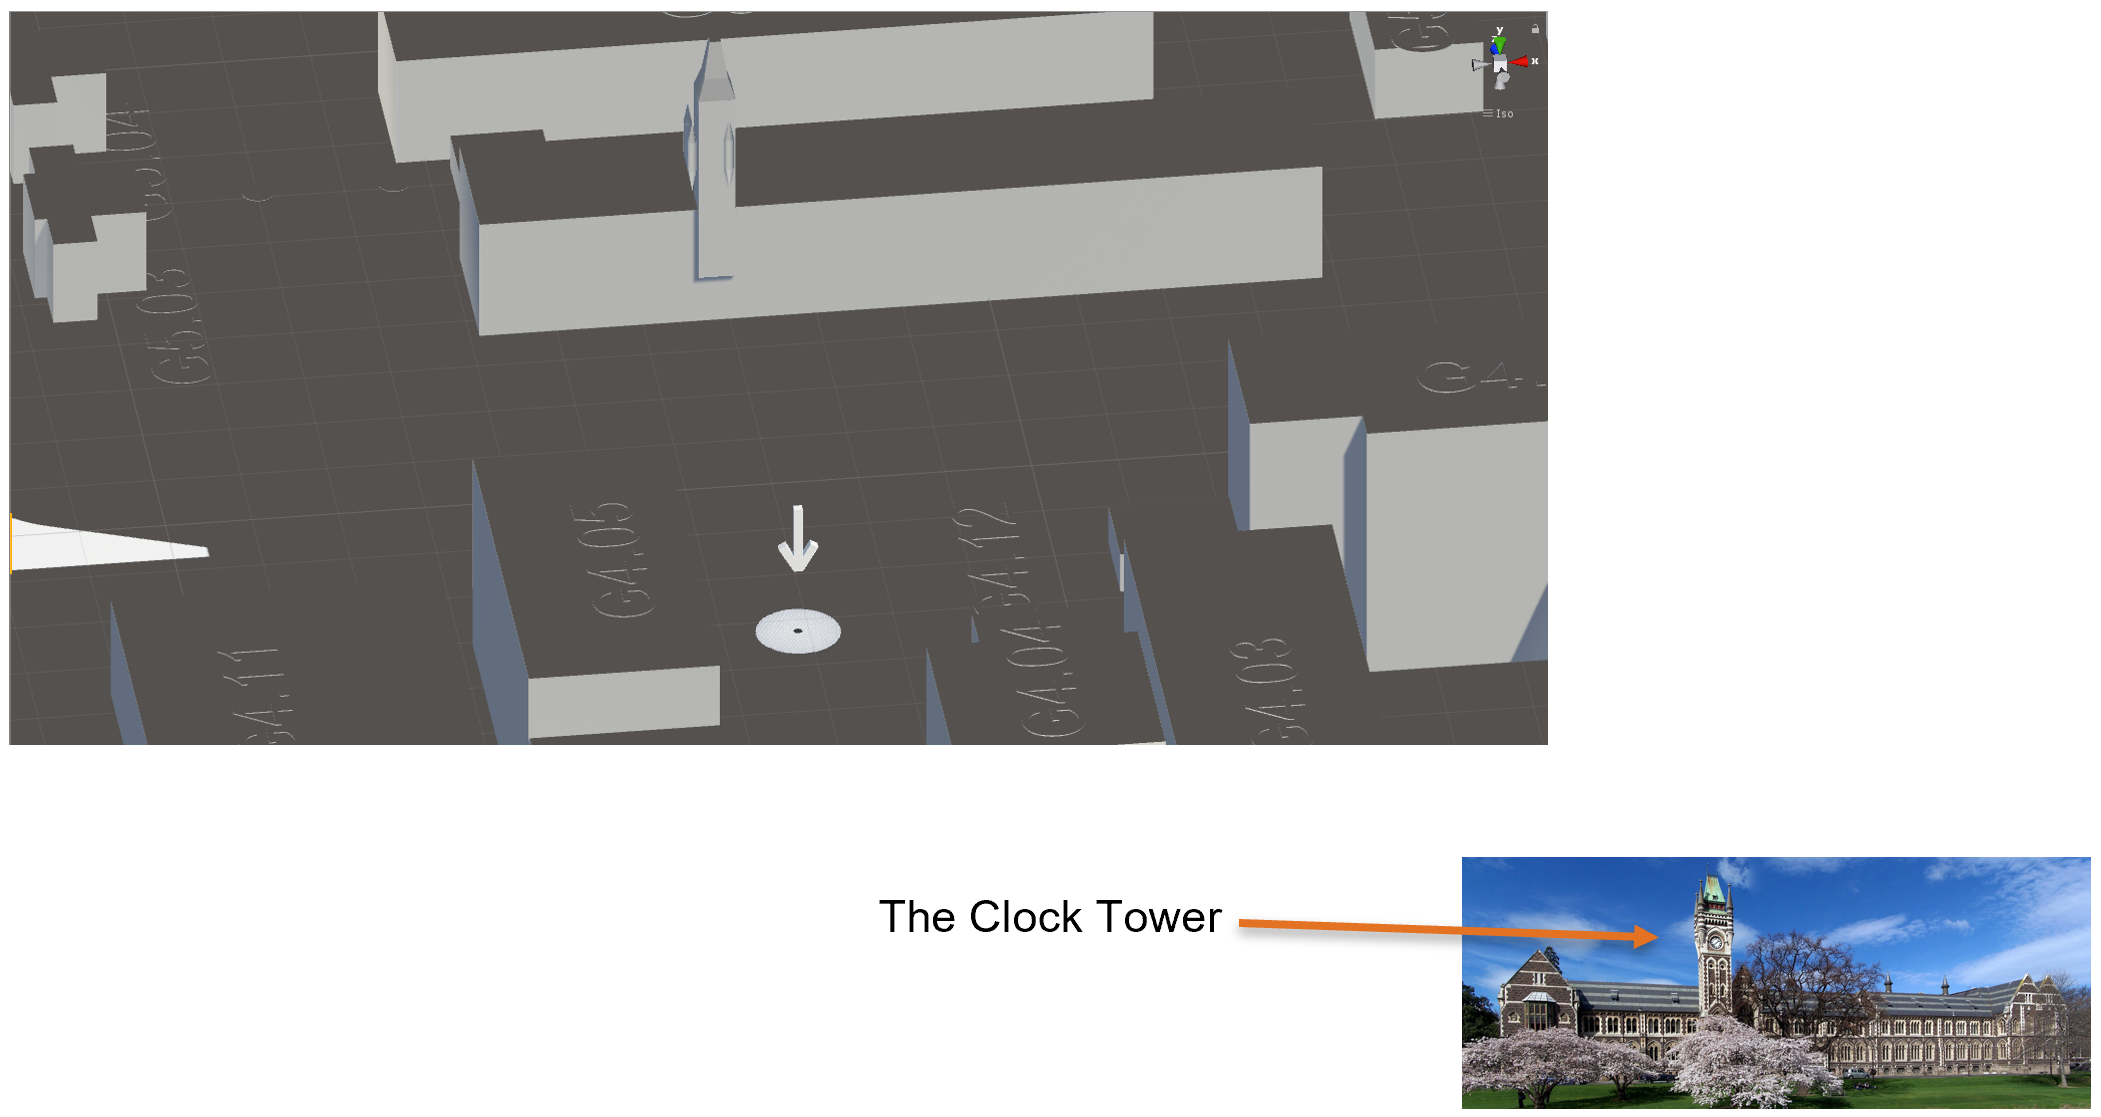
\includegraphics[width=0.7\linewidth]{figures/placeholders/prototype2_viewving_spot}
	\caption{The viewing spot in-front of the university clock tower}
	\label{fig:prototype2viewvingspot}
\end{figure}
\begin{figure}
	\centering
	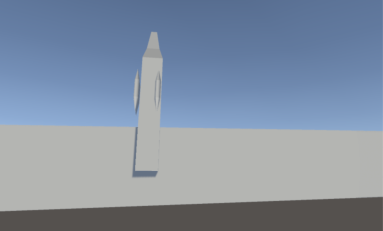
\includegraphics[width=0.7\linewidth]{figures/placeholders/prototype2_clocktower_odd_features}
	\caption{The odd features of the university clock tower model}
	\label{fig:prototype2clocktoweroddfeatures}
\end{figure}

% Apparatus
%The same apparatus was used, as in the \nameref{buildingspoppingup} prototype.

% Results
The participants' feedback about the experience was variable: two (one with good, and one with little experience with \gls{vr}) indicated that the building approaching them was an unpleasant experience, one of them said he was startled by it. The other two participants indicated that the experience was "not scary". One of them thought that this was due to the building moving to slow. Two participants reported thinking that the moving building was a result of them pressing a button or a tracking error.	

% Limitations
In spite of the informal nature of the preliminary prototype experiments, the results indicated disagreement among the participants, and the problem was deemed worthy of further exploration.


\section{Pilot Studies}
After the research into sonification and awareness, and after the vision for the final \nameref{final_study} study was established, two pilot studies were conducted, \nameref{study_one} and \nameref{study_two}. This was done in order to study certain aspects of the final study separately, and make decisions, such as what sound type (abstract earcons or auditory icons) to choose, at what speed to translate the buildings, and whether stereo headphones are suitable for the planned system.

\subsection{Sound Speed and Type}
\label{study_one}
% Goal of the study
Feedback from the initial prototypes indicated that the speed of the moving building was too slow. The goal of this study was to derive the speed participants felt comfortable with, and that would allow them to make correct spatial judgments. Additionally, this pilot study was meant to determine what type of audio feedback to use: abstract earcons or auditory icons.

\paragraph{Participants}
Eight participants (7 men, 1 woman) were chosen among the members of the \gls{hci} group at the University of Otago, New Zealand. One had reported bad hearing, and one had a flu.  None of the participants had any architectural background, some were online gamers.

\paragraph{Procedure \& Task}
The study was carried out in a \gls{ve} that was specifically constructed for this purpose (see Fig. \ref{fig:clipimage001}). A participant would be placed at the Center (C) of the environment. A real-sized building, approximated with a cuboid, was present in the environment. It could be translated by the experimenter from and to any of the predefined positions: Left Front (LF), Right Front (RF), Left Back (LB), Right Back (RB), Front (F), Back (B), Left (L), Right (R), C. When the building moved, it would emit sound.

Participants were instructed with the purpose the research, this study, and the tutorial, as well as their individual task. Participants were placed at the center of the scene (C) with the building placed in front of them, and asked to preserve the orientation of the chair they were seated upon, but were also told that they were allowed to move their head.

Participants were put through a tutorial to build a correlation between the visually perceived movements of the building and the emitted sound: the building was translated along the major directions (C-F, C-L, L-R, L-C, C-B), and then additionally between randomly selected positions from the predefined set (Fig. \ref{fig:pilot1predefinedtutorialtranslations}).

At the start of the actual experiment, participants were asked to close their eyes and guess the path that the building traversed. It was silently positioned at a randomly selected position and then translated, with audio feedback turned on, to a newly selected random position (see Fig. \ref{fig:arbitrary_translation}). This was repeated 5 to 10 times for each of 6 type of sound-speed combinations.

After going through all the sound types and speeds, participants were asked for their honest opinion, as to which sound was the best, and what speed was the most appropriate.

\begin{figure}
	\centering
	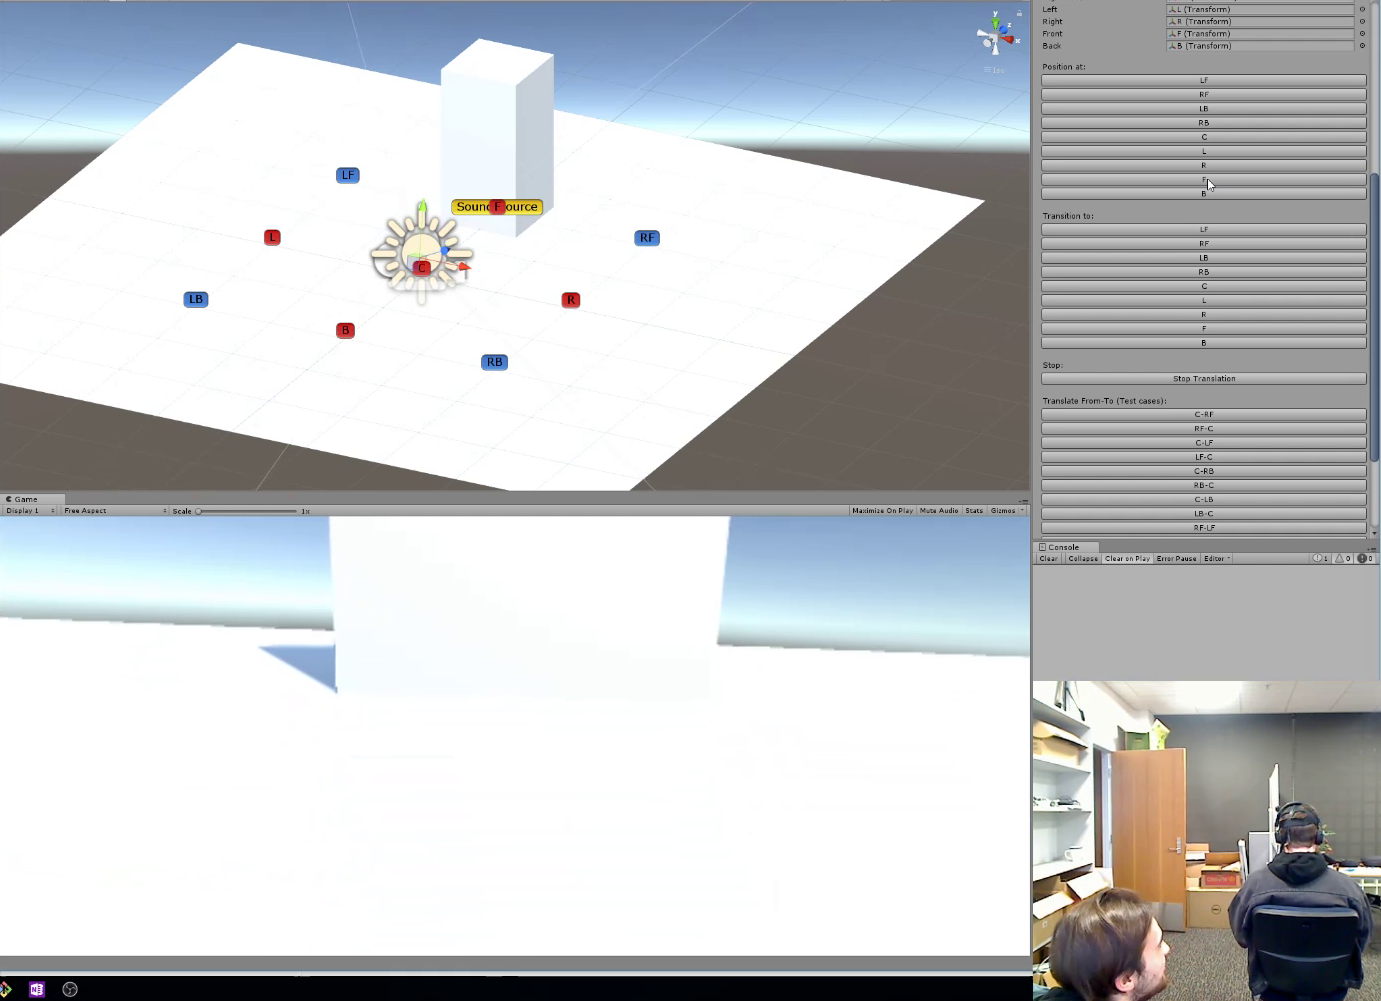
\includegraphics[width=0.7\linewidth]{figures/placeholders/pilot1_experiment_setup.png}
	\caption{Experiment setup}
	\label{fig:clipimage001}
\end{figure}

\begin{figure}
	\centering
	\subfloat[Predefined translation paths]{
		\label{fig:pilot1predefinedtutorialtranslations}
		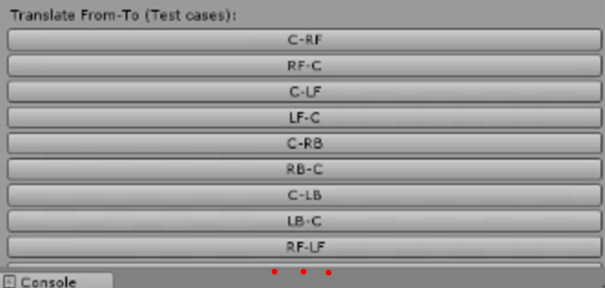
\includegraphics[width=0.3\linewidth]{figures/placeholders/pilot1_predefined_tutorial_translations}
	} %

	\subfloat[Arbitrary translations]{
		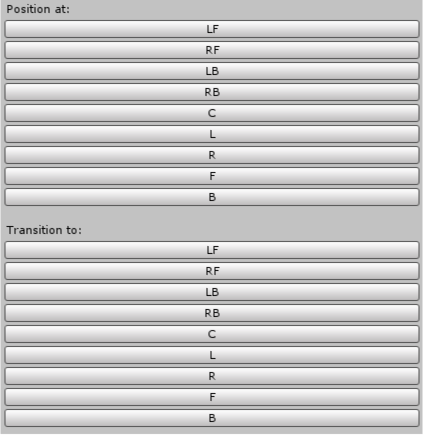
\includegraphics[width=0.3\linewidth]{figures/pilot1_control_panel}
		\label{fig:arbitrary_translation}
	}
	
	\caption{Control panels}
	\label{fig:pilot1controlpanel}
\end{figure}


\paragraph{Apparatus}
% Apparatus (i.e Unity, Resonance Audio, stereo headphones, Vive)
Experiment was implemented with the help of Unity3d  2018.1.5f1 and Resonance Audio SDK for Unity, version 1.2.1 with sound occlusion turned off. For the hardware, HTC Vive \gls{vr} headset, along with on-ear stereo headphones, and a Windows 10 PC.
Audacity 2.2.2 was used prior to the experiments to: mixdown stereo sounds to mono, make audio tracks seamless, and increase the volume.

% Study Factors and Conditions: what my factors are, conditions == independent variables' values
\paragraph{Study design}
The study followed the repeated measures design with 2 independent variables: translation speed and different types of audio feedback.

Three different translation speeds were tested: \textit{slow} - 20, \textit{medium }- 40, and \textit{fast }- 60 meters per second (m/s). Sound properties (i.e. pitch, playbackspeed) stayed constant throughout the different speeds.

Two different types of the audio feedback were tested: earcons and auditory icons. A full volume 100 Hz sine wave in mono was used for an earcon (Type: Wave (.wav), Samplerate: 44100.0 Hz, Bitdepth: 16bit, Fig. \ref{fig:pilot1sinewaveedit}). As an auditory icon a mono sound mimicking moving concrete block with sound amplitude extrema reaching full volume was used (Type: Wave (.wav), Samplerate: 48000.0 Hz, Bitdepth: 16 bit, Source: https://freesound.org/people/FreqMan/sounds/25846/, Fig. \ref{fig:pilot1concreteonconcretesoundedit}).
The type of sound played first was rotated for the participants, so that 4 of them heard the auditory icon first, and the other 4 - the earcon.

\begin{figure}
	\centering
	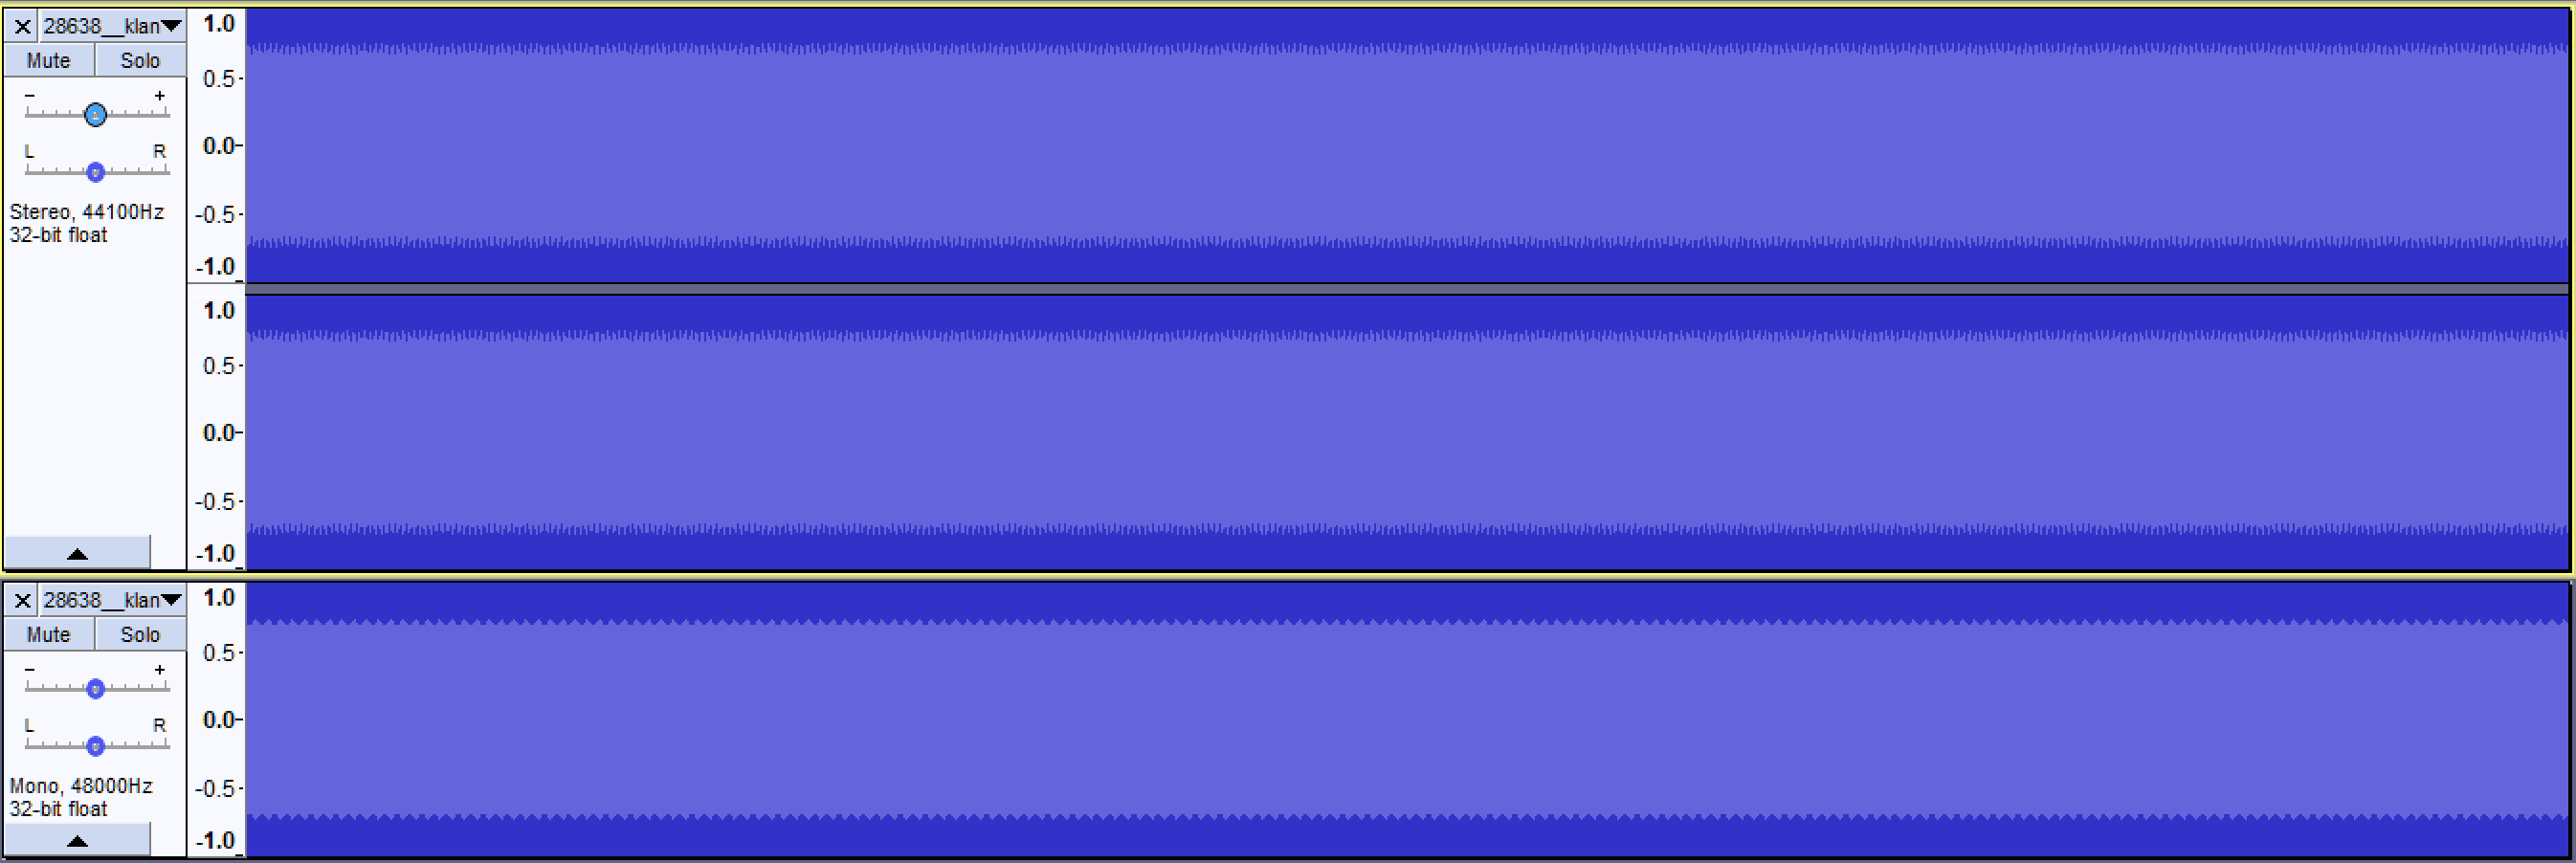
\includegraphics[width=0.7\linewidth]{figures/pilot1_sinewave_edit}
	\caption{Sine wave earcon before (top) and after (bottom) mixdown: stereo to mono}
	\label{fig:pilot1sinewaveedit}
\end{figure}

\begin{figure}
	\centering
	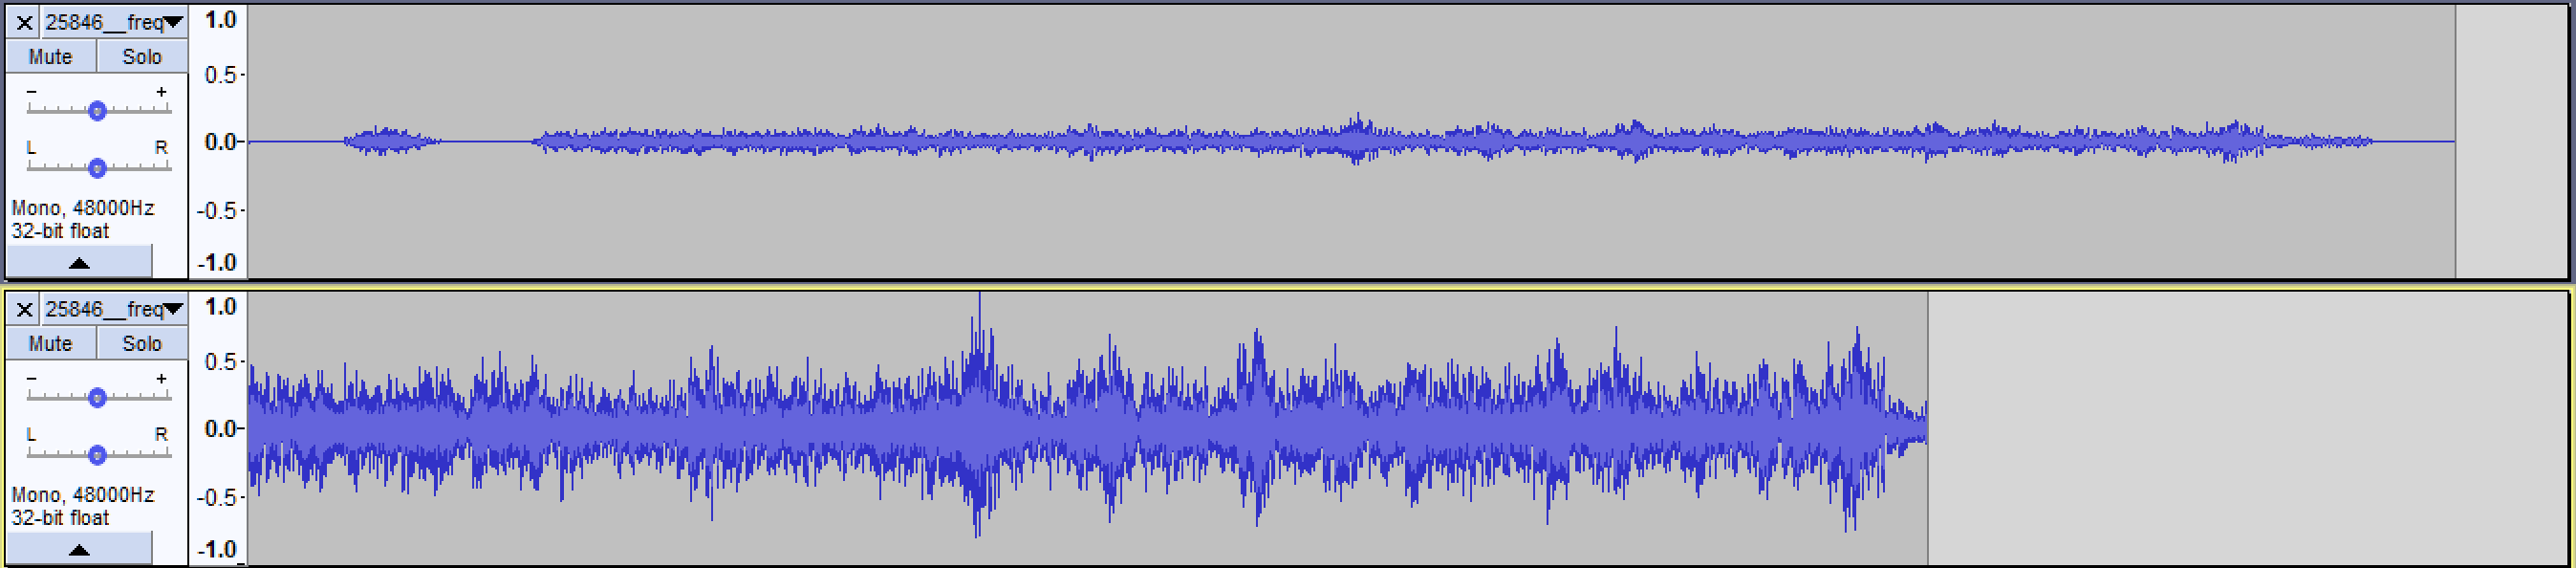
\includegraphics[width=0.7\linewidth]{figures/pilot1_concrete_on_concrete_sound_edit}
	\caption{Concrete sliding on concrete auditory icon before (top) and after (bottom) amplification, and crop}
	\label{fig:pilot1concreteonconcretesoundedit}
\end{figure}

Translations were pseudo-randomized across participants, their selection was made with some degree of bias towards longer translation paths, so that users have more time to analyze the sound and guess (i.e. the path from RB to LB would be longer, than just RB to B). Different translation paths can be seen in Fig. \ref{fig:pilot1translationpaths}.

Distances between the fixed translation end-points remained the same throughout the experiment: 20 Unity3d units (meters) between C-F, C-L, C-R, C-B, L-LB, and so on.

\paragraph{Results} \hfill

\textit{Preferred sound} 6 out of 8 participants preferred the concrete sound to the sine wave, 1 was indifferent as long as the speed was slow, and 1 preferred the sine wave.

\textit{Preferred speed} The speed preference can be seen in the Table \ref{table:pilot1_results}.

\begin{figure}
	\centering
	
	\subfloat[Top-down view of the scene]{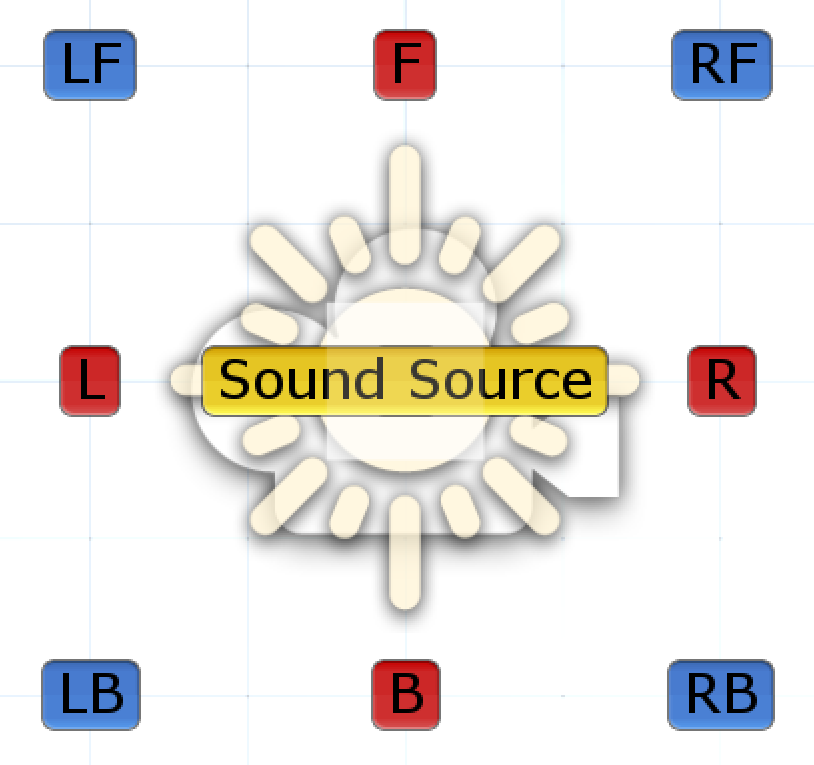
\includegraphics[scale=.4]{figures/pilot1_top_down_scene_view.png}}%
	\subfloat[Major translation paths]{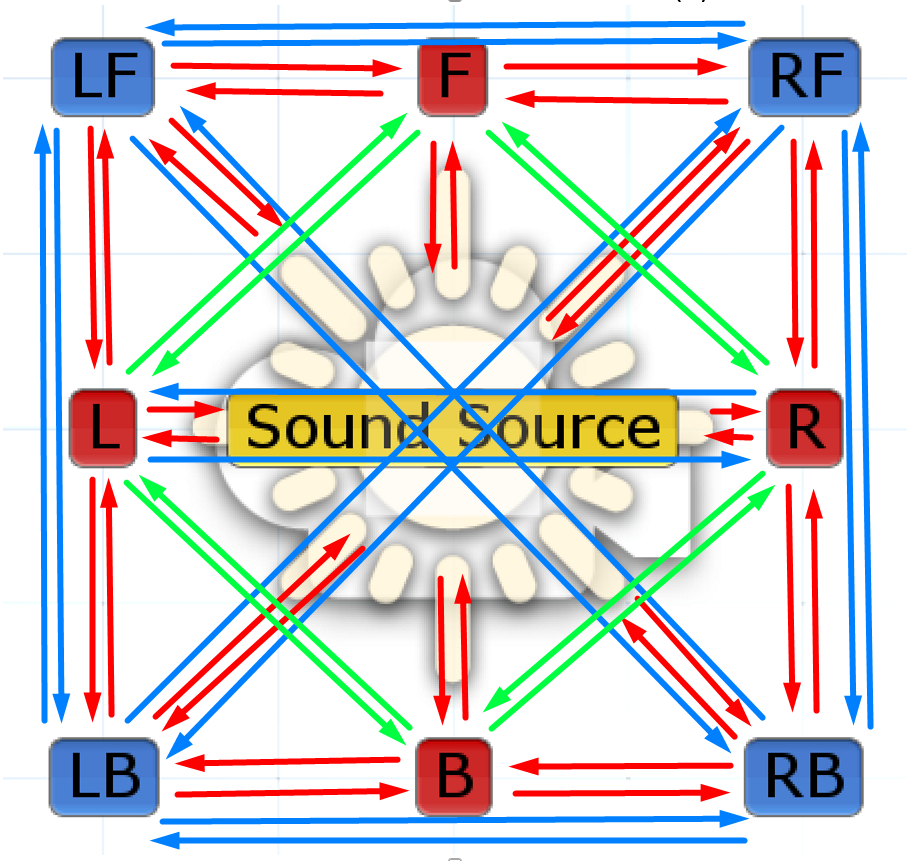
\includegraphics[scale=.4]{figures/pilot1_top_down_scene_view&major_tranlsation_paths.png}}%
	\subfloat[All translation paths]{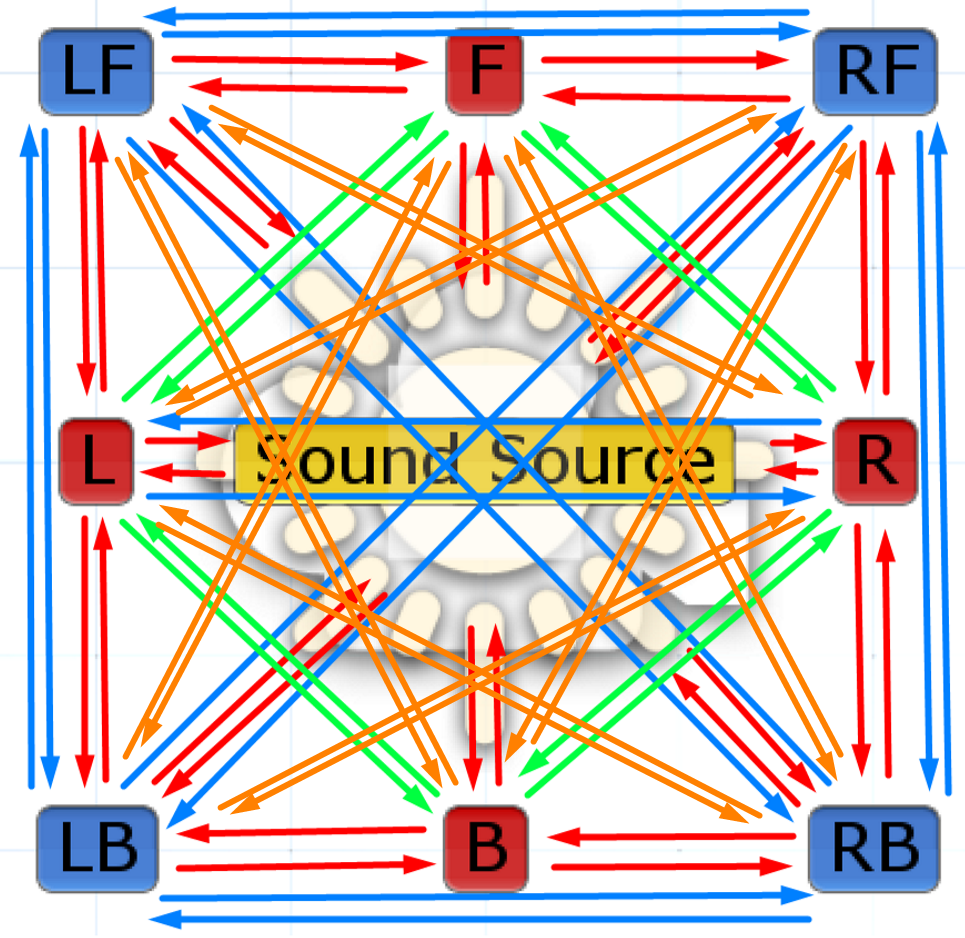
\includegraphics[scale=.4]{figures/pilot1_top_down_scene_view&all_possible_translation_paths.png}}
	
	\caption{Possible translation end-points and paths}
	\label{fig:pilot1translationpaths}
\end{figure}


\begin{table}[h]
	\label{table:pilot1_results}
	\caption{Experiment data}
	
	\begin{tabularx}{\linewidth}{|l|l|l|X|}
		\hline
		\textbf{Participant} & \textbf{First sound played} & \textbf{Preferred sound} & \textbf{Preferred speed}                        \\ \hline
		1                    & Concrete                    & Concrete                 & Medium                                          \\ \hline
		2                    & Concrete                    & Concrete                 & Slowest, then medium                            \\ \hline
		3                    & Sine wave                   & Concrete                 & Medium                                          \\ \hline
		4                    & Sine wave                   & Concrete                 & First two - fine (fastest one - a bit too fast)  \\ \hline
		5                    & Concrete                    & Either                   & Slowest                                         \\ \hline
		6                    & Sine wave                   & Sine wave                & Fast (speed didn't affect it too much)          \\ \hline
		7                    & Concrete                    & Concrete                 & Between slow and medium                         \\ \hline
		8                    & Sine wave                   & Concrete                 & First two - fine (fastest one - a bit too fast) \\ \hline
	\end{tabularx}
\end{table}

\paragraph{Discussion}
If we visualize the participants' preferences, and take the smallest common area, where they overlap, analysis shows that participants preferred the speed somewhere close to 40 m/s, but between 20 and 40 (Fig. \ref{fig:pilot1resultsanalysis})

The choice of the sound was most likely caused by its natural fit to the ecology of the system - users expect a sound similar to the concrete on concrete auditory icon when they see a large cuboid sliding on the stone floor. However, if we consider the attributes of the chosen sounds, the auditory icon would almost always be a better choice, if simply due to fact that it has a distinct timbre with its harmonics and overtones. On the other hand, the chosen abstract earcon was a simple "timbreless" sine wave, which might make it harder to memorize.
Additionally, in we consider sound occlusion (which was turned of in all studies), the audio spatialization SDK that I use in this experiment implements it through filtering out low-frequency component of a sound wave. And since sine wave is a single-component wave, a cases where the sound is completely masked can occur.

\begin{figure}	
	\centering
	
	\subfloat["Medium"]{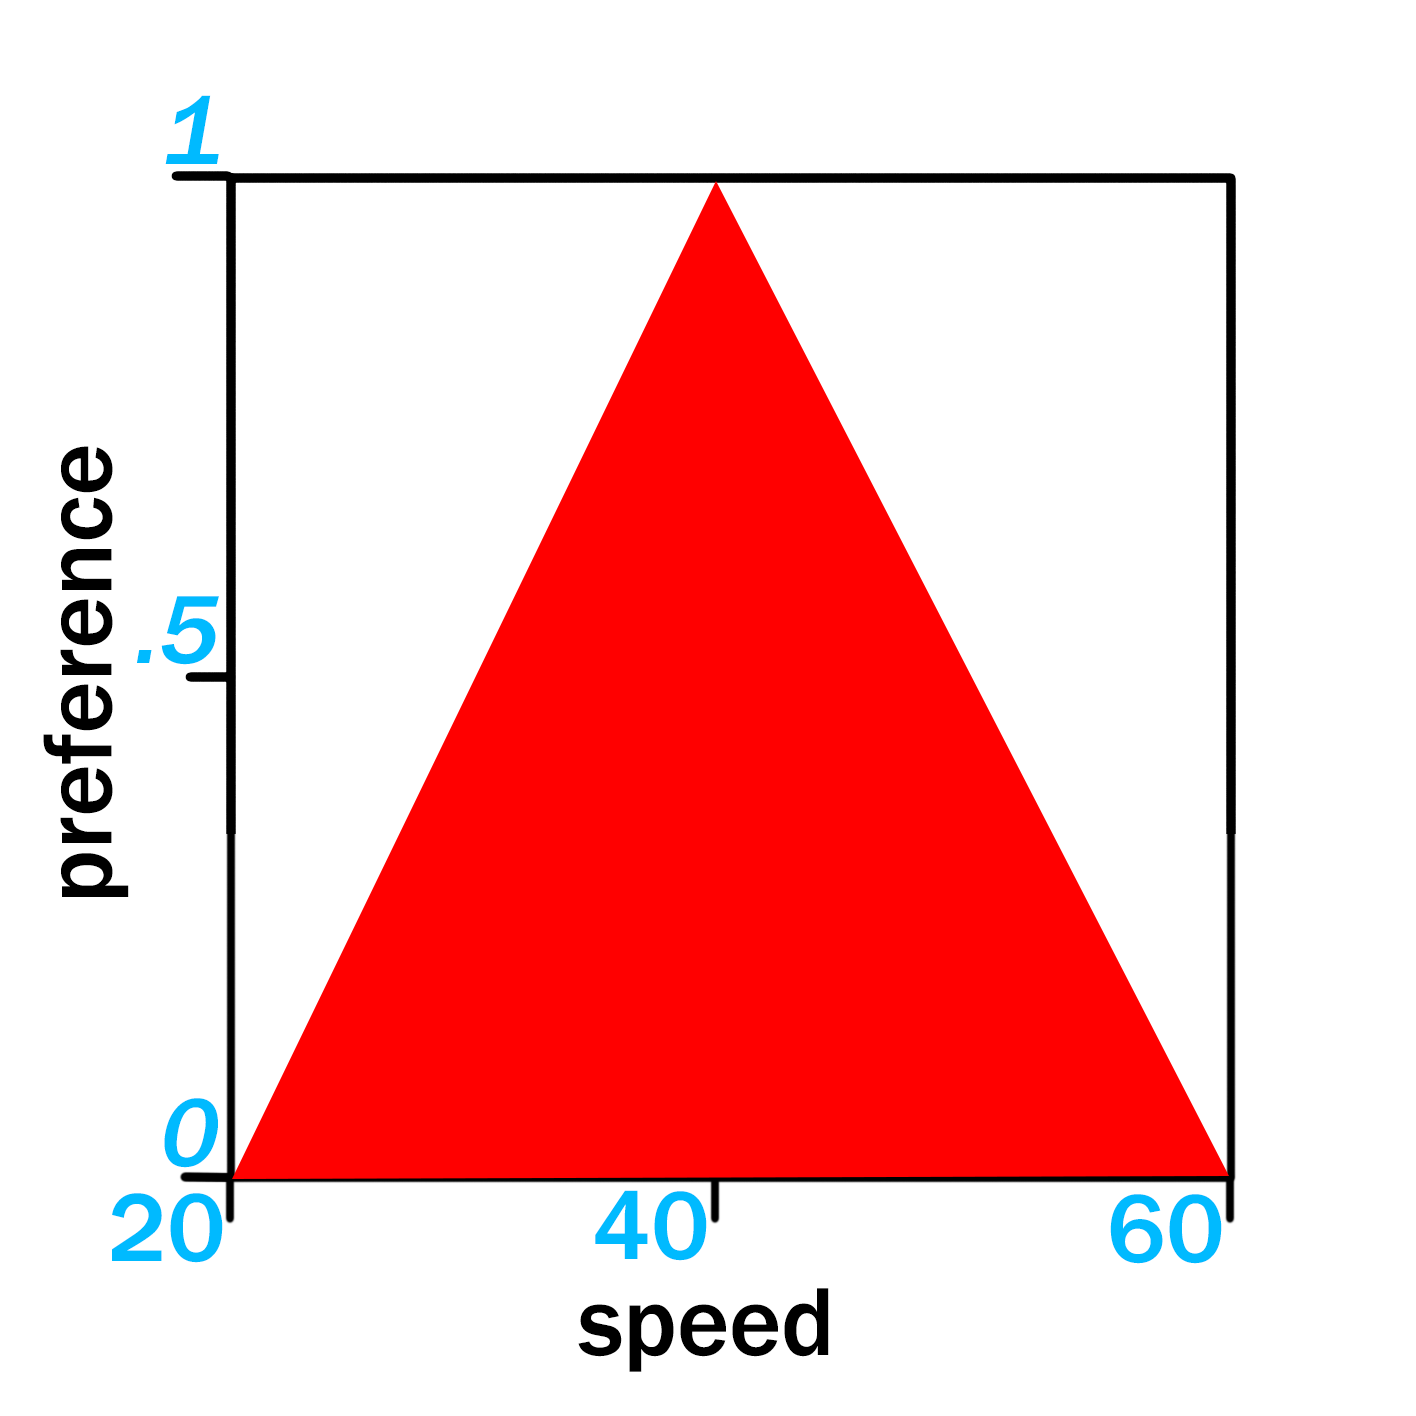
\includegraphics[scale=.075]{figures/pilot1/results/speed_fuzzy_preference_medium.png}}%
	\subfloat["Slowest, then medium"]{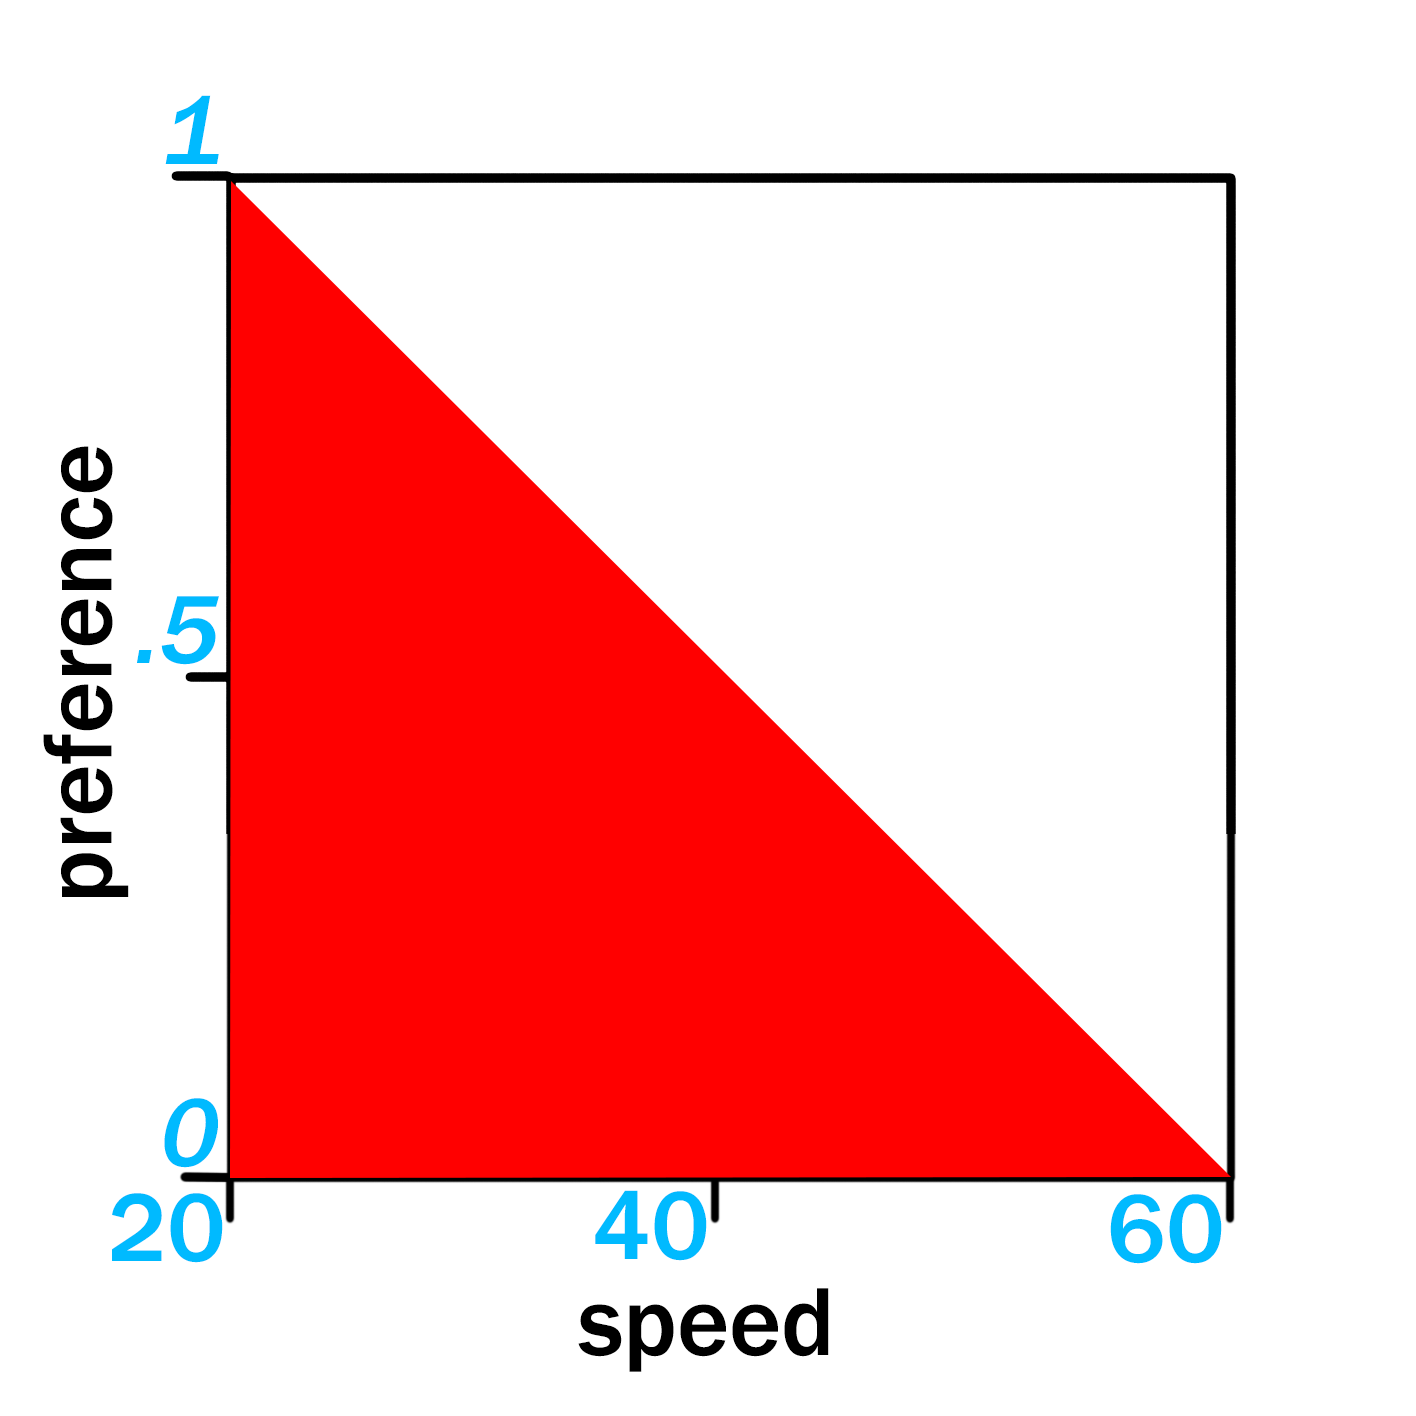
\includegraphics[scale=.075]{figures/pilot1/results/speed_fuzzy_preference_slowest_then_medium.png}}%
	\subfloat["First two - fine..."]{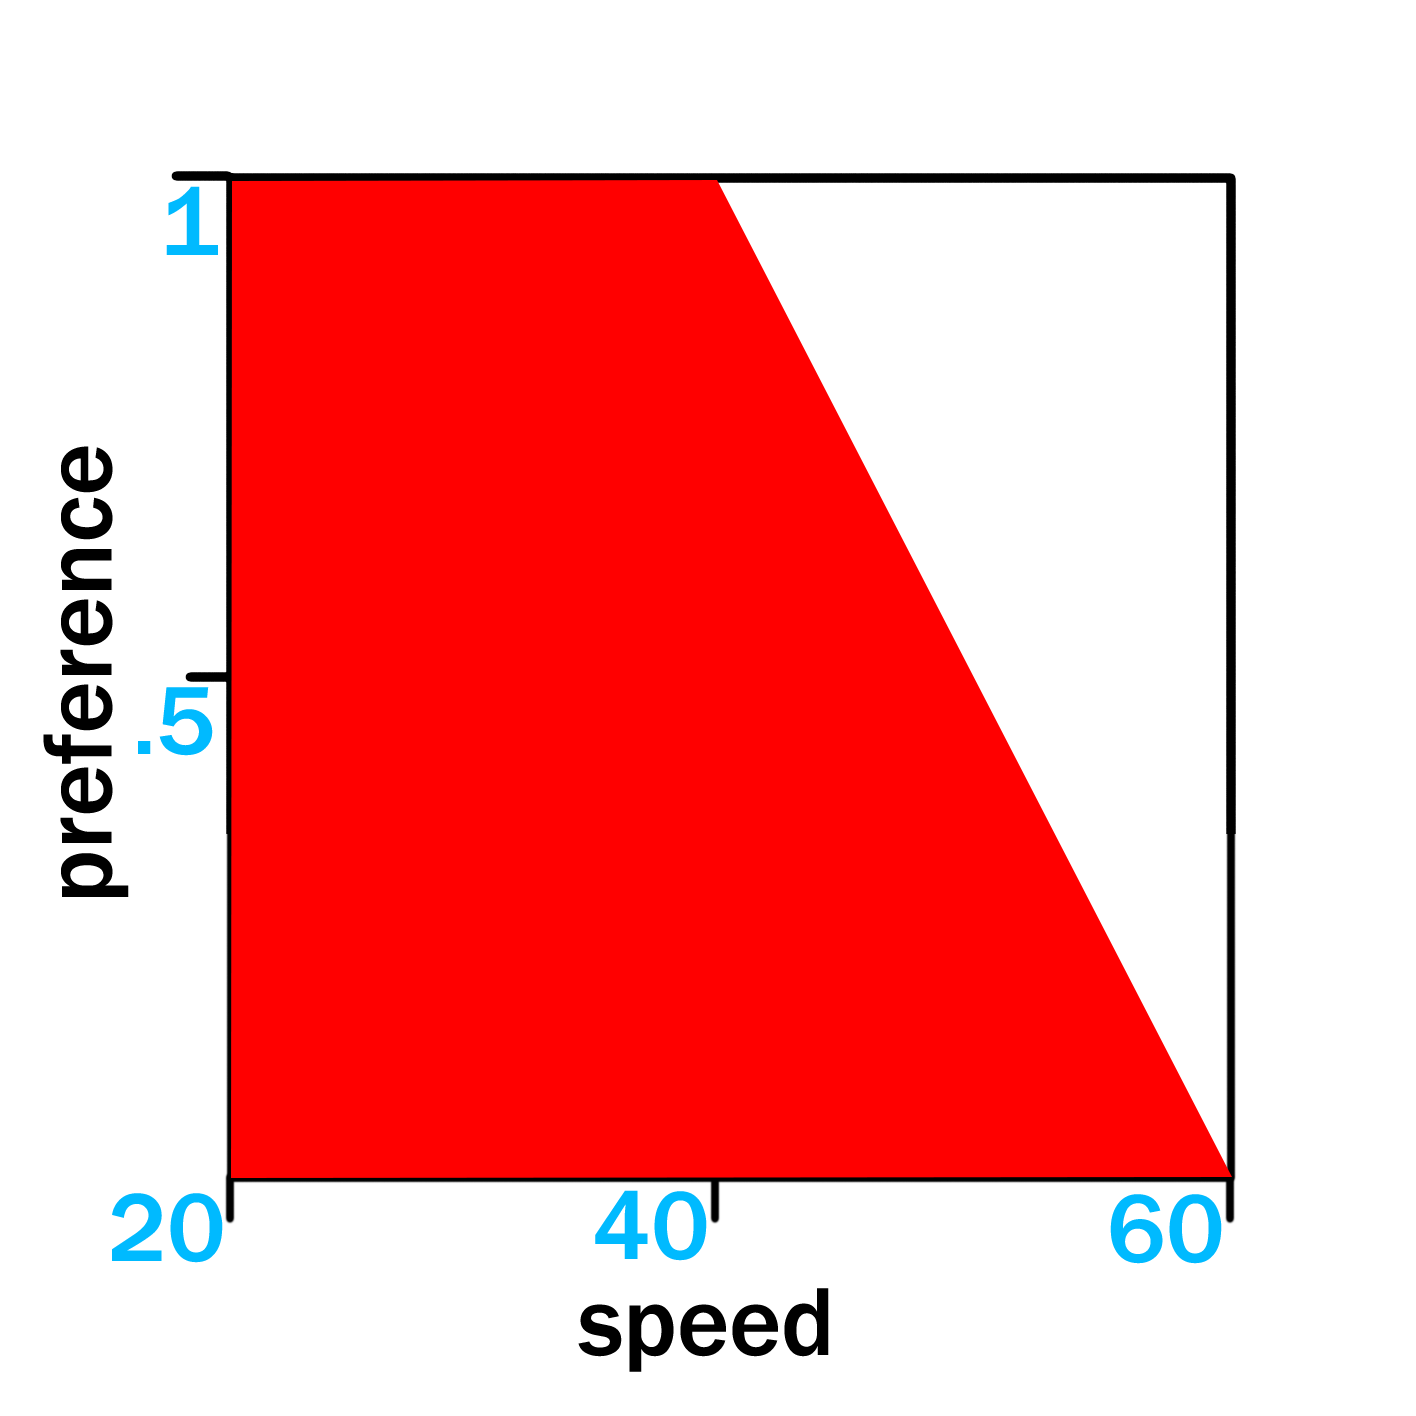
\includegraphics[scale=.075]{figures/pilot1/results/speed_fuzzy_preference_first_two_fine.png}}%
	\subfloat["Slowest"]{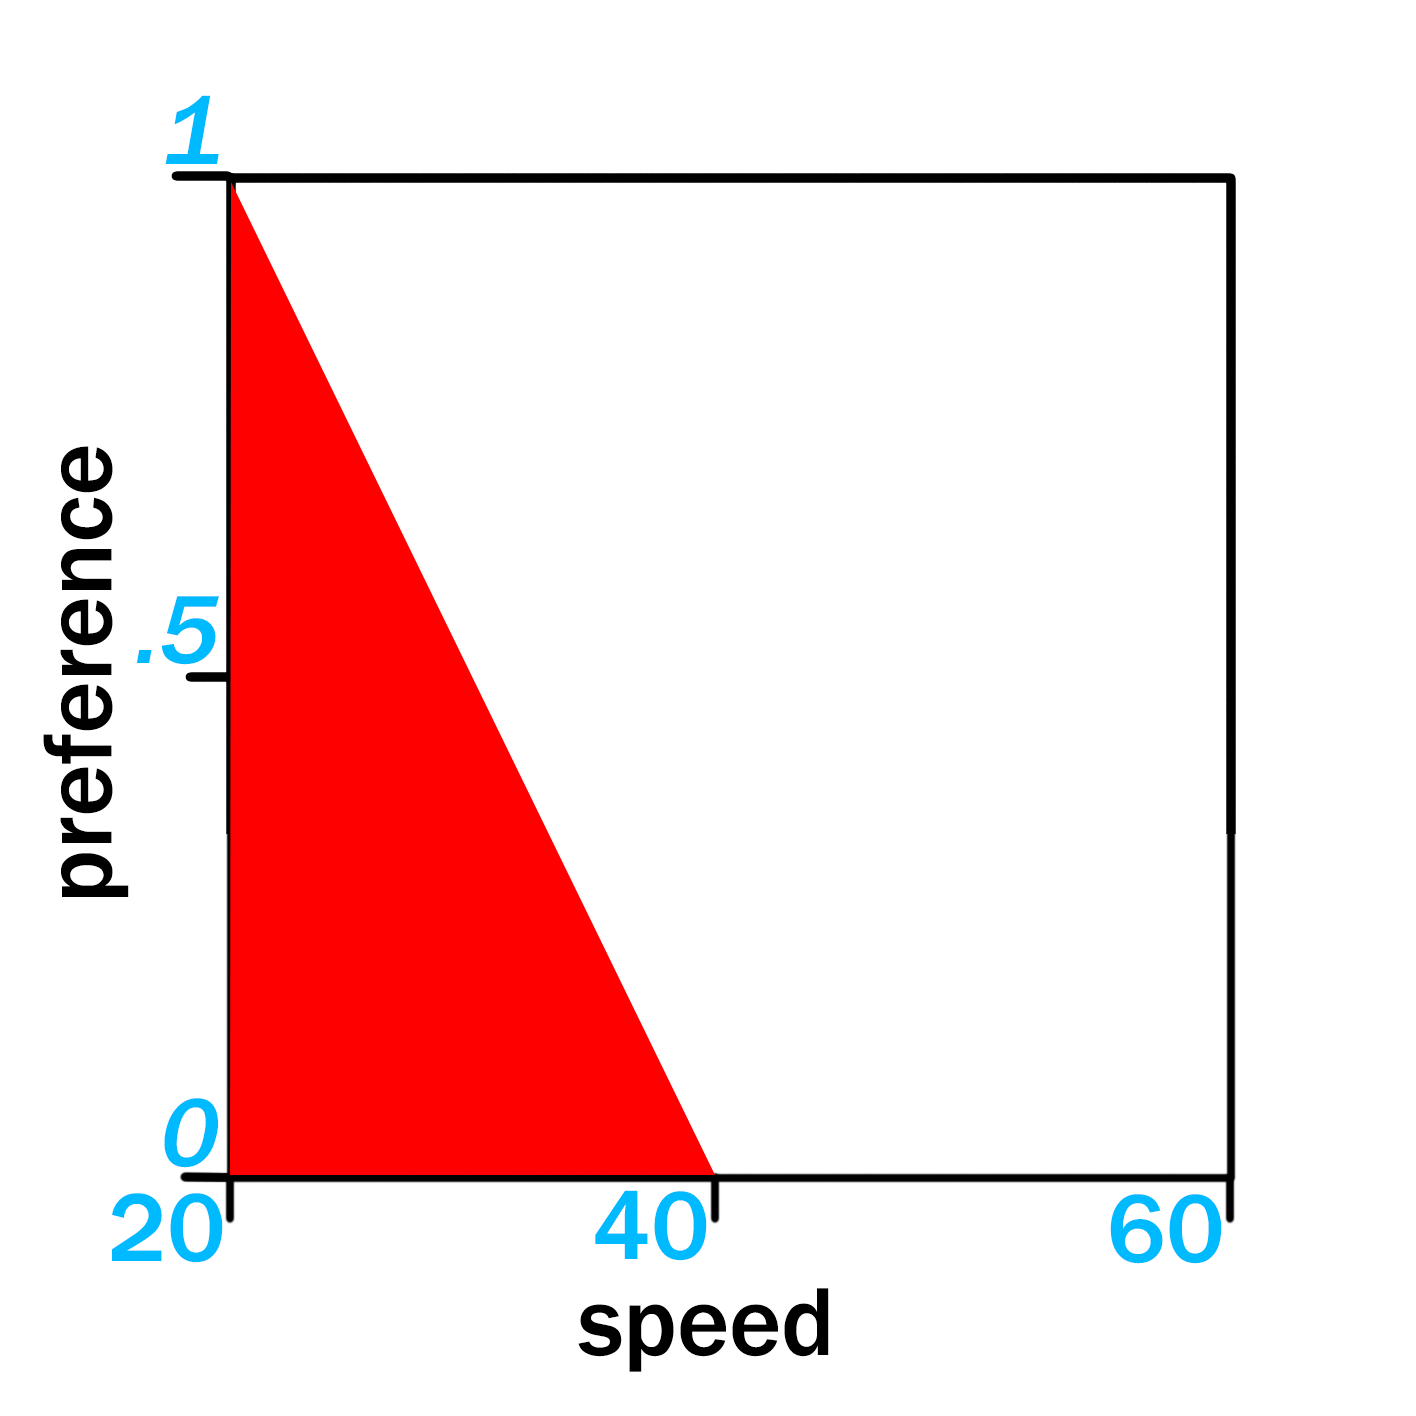
\includegraphics[scale=.075]{figures/pilot1/results/speed_fuzzy_preference_slowest.png}}
	
	\par\medskip
	\subfloat["Fast..."]{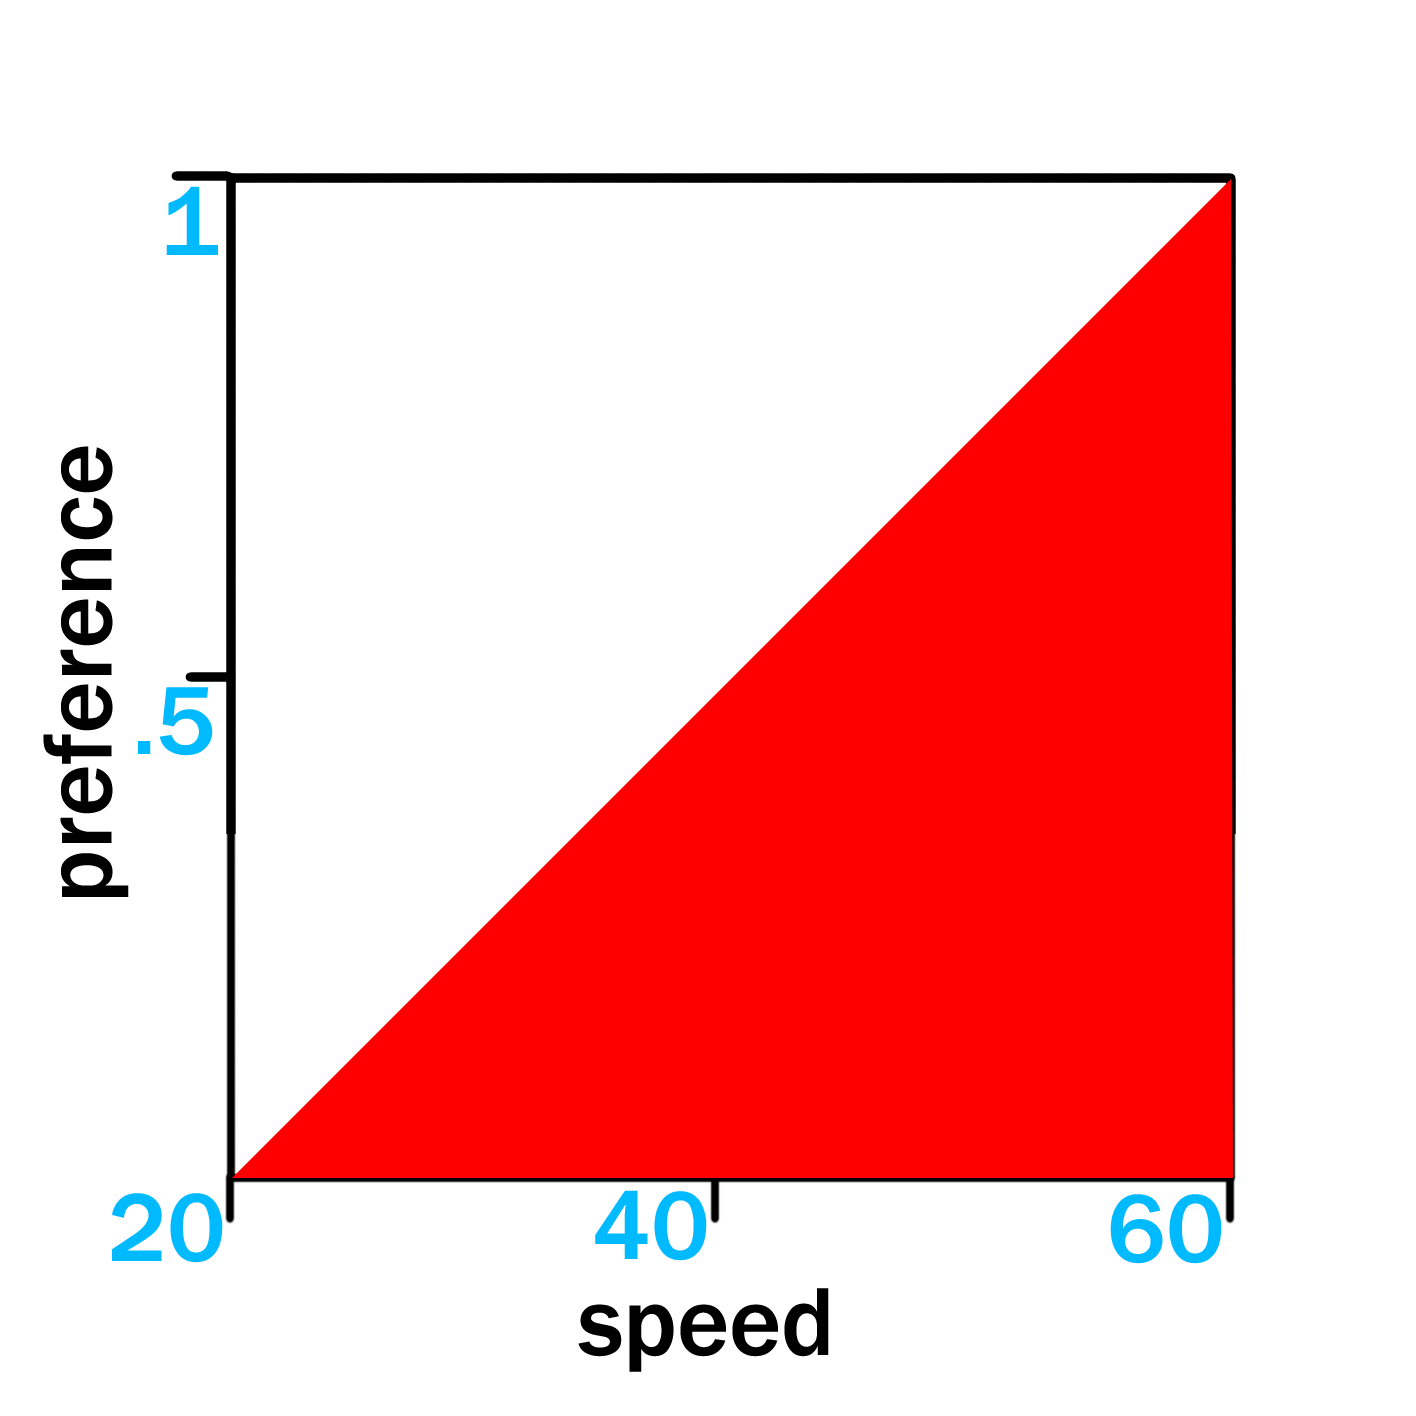
\includegraphics[scale=.075]{figures/pilot1/results/speed_fuzzy_preference_fast.png}}%
	\subfloat["Between slow and medium"]{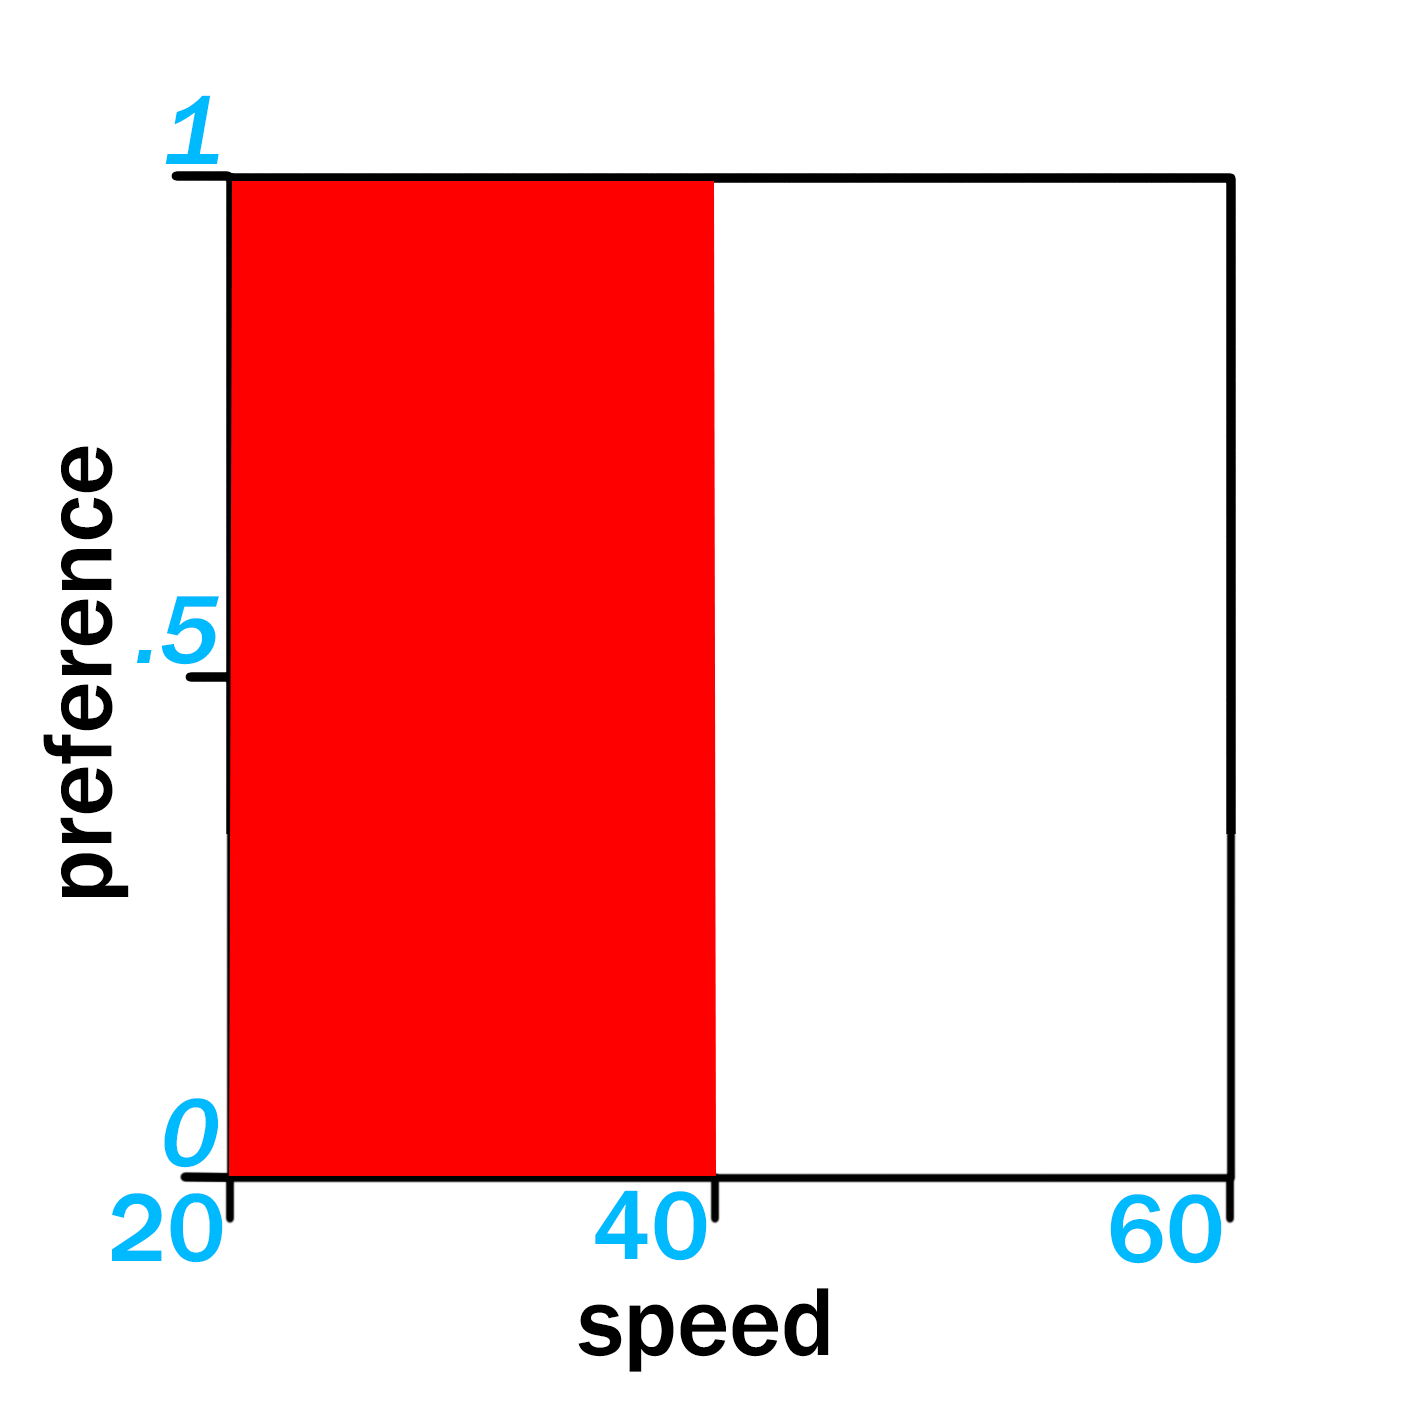
\includegraphics[scale=.075]{figures/pilot1/results/speed_fuzzy_preference_between_medium_and_slow.png}}%
	\subfloat[Answers combined with 12\% opacity each]{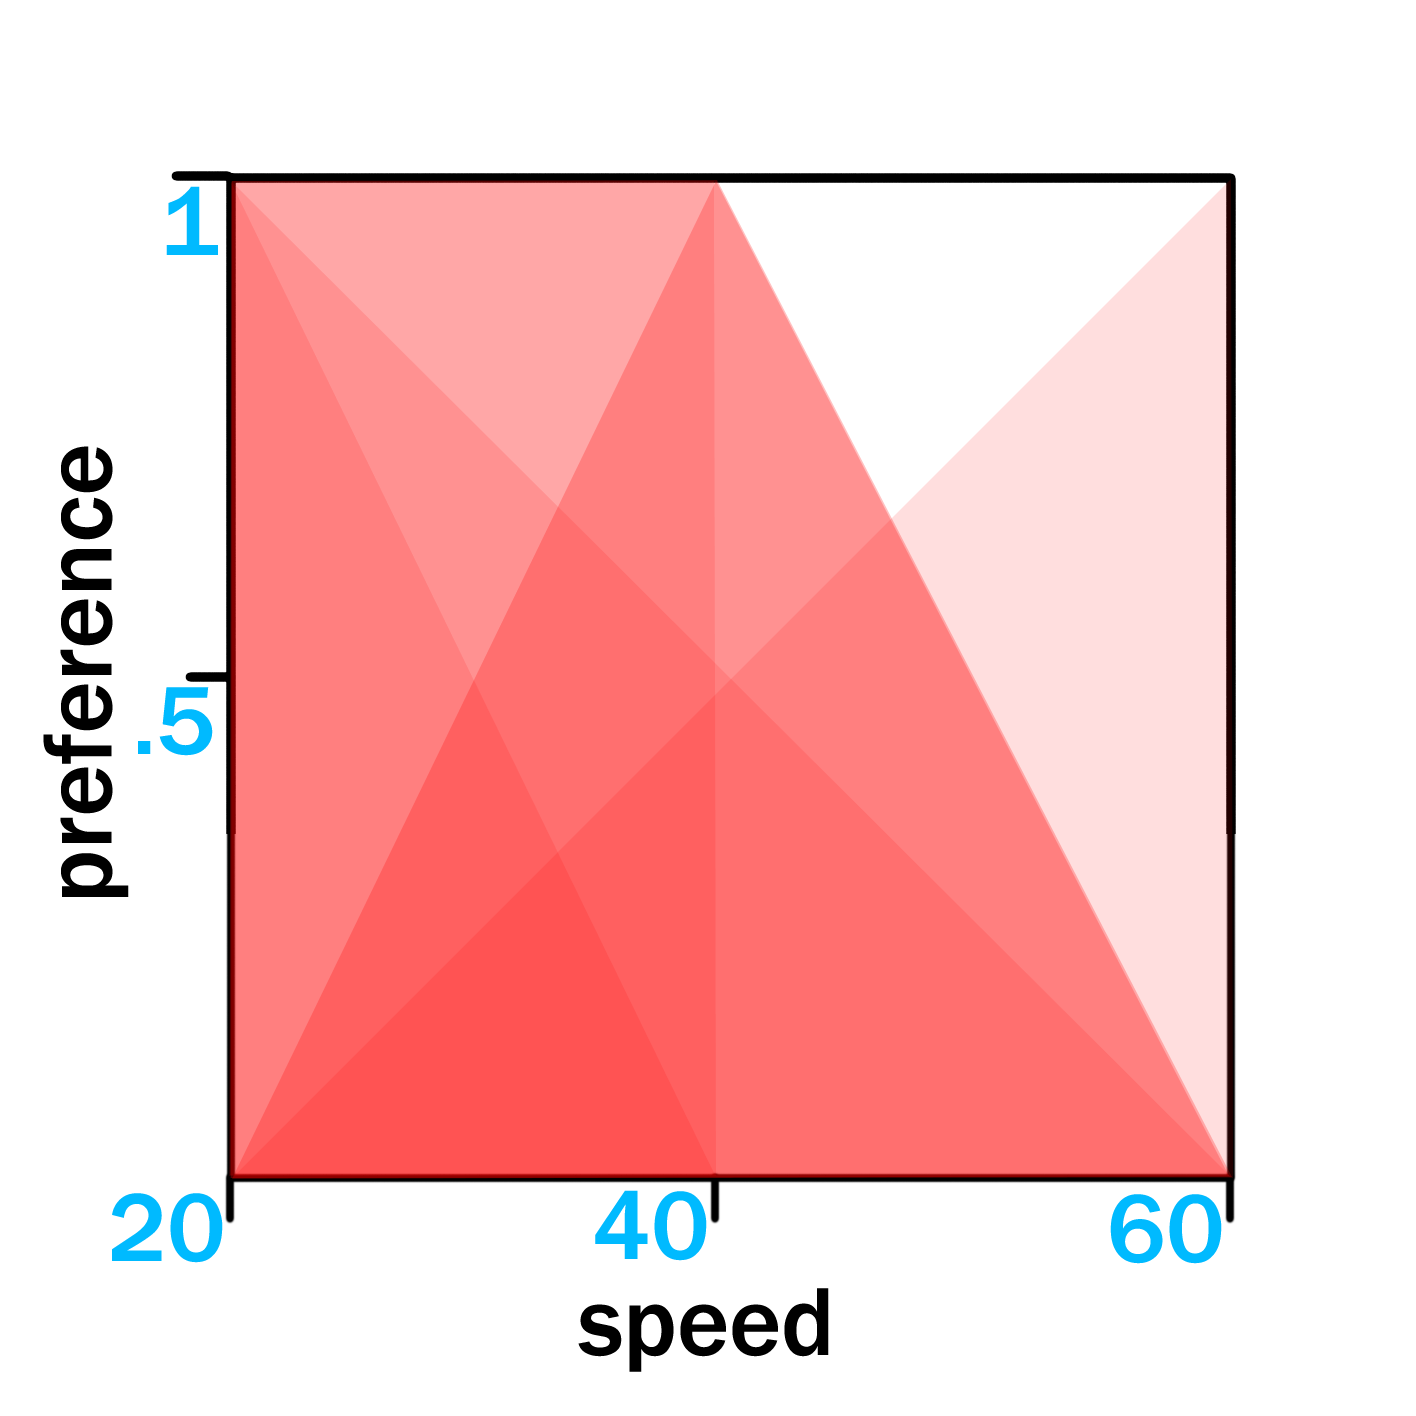
\includegraphics[scale=.075]{figures/pilot1/results/speed_fuzzy_preference_result_no_highlight.png}}	
	
	\par\medskip
	\subfloat[Preferred speed according to analysis]{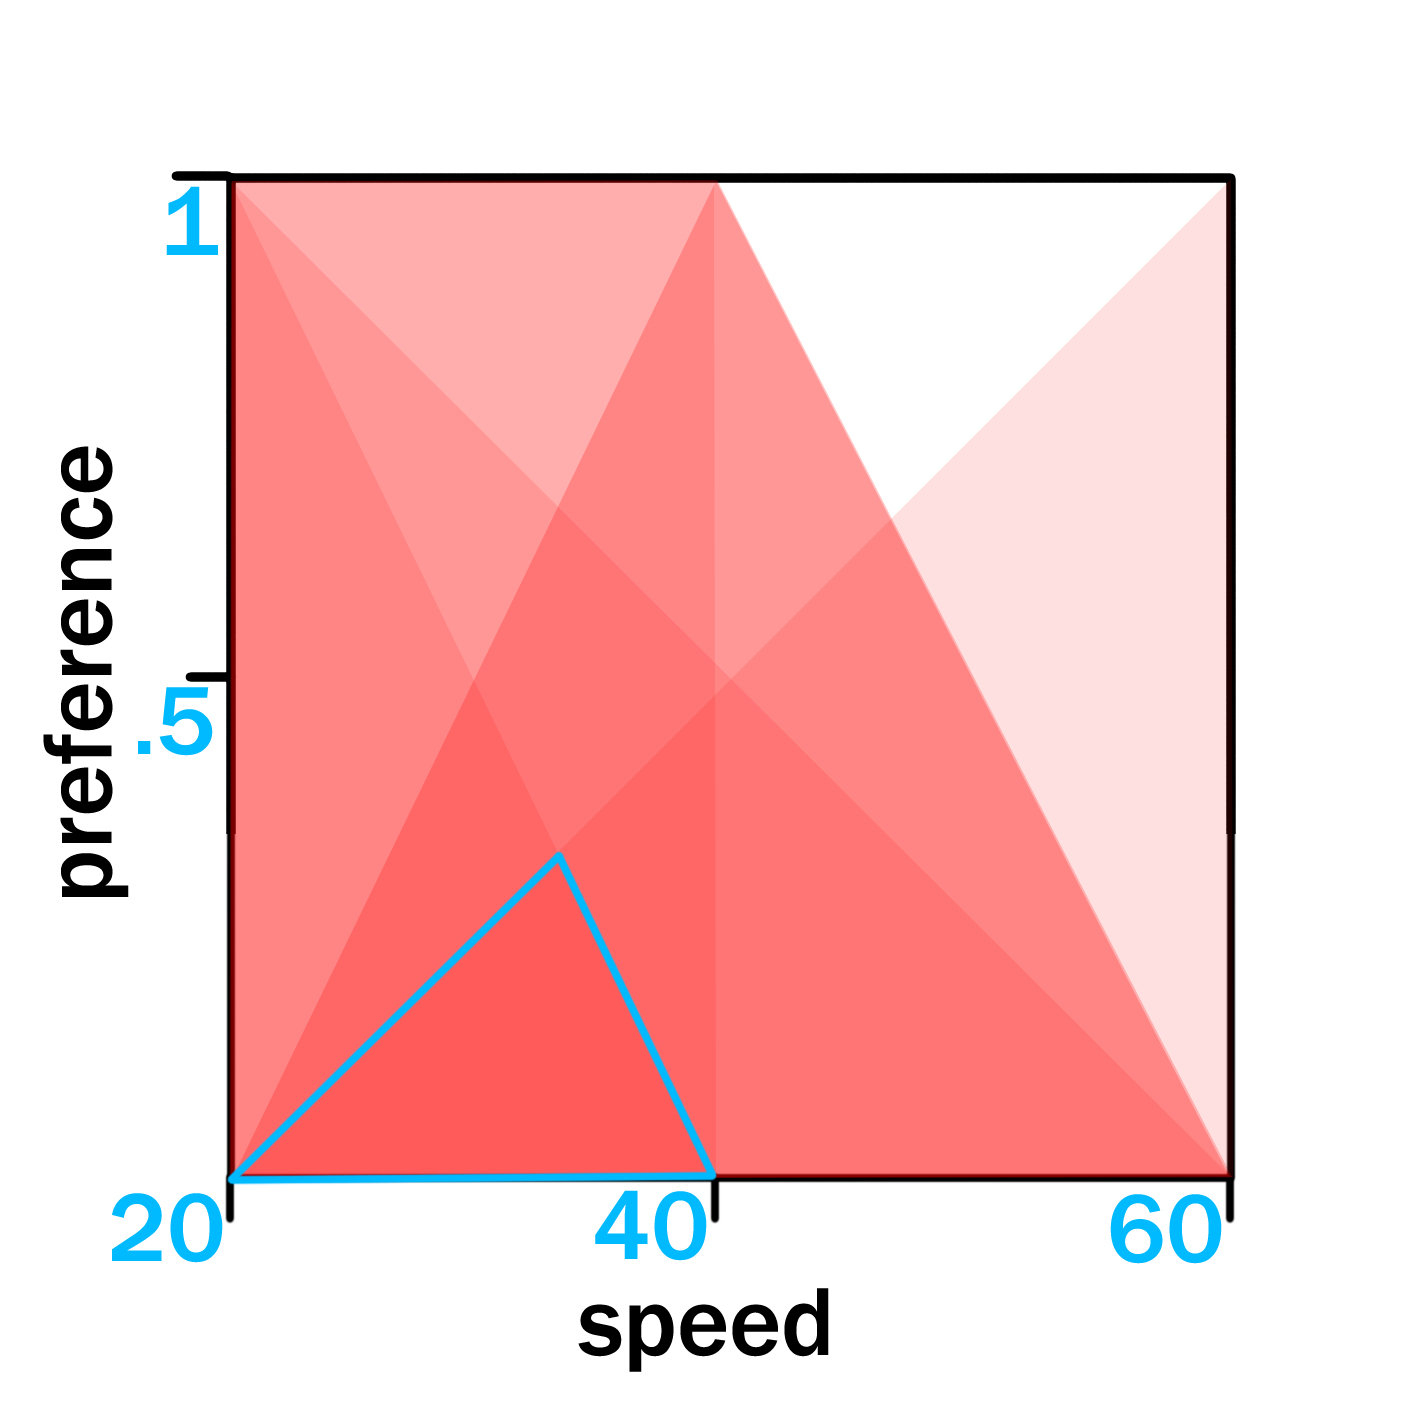
\includegraphics[scale=.15]{figures/pilot1/results/speed_fuzzy_preference_result.png}}
	
	\caption{Visual analysis of results, pilot 1}
	\label{fig:pilot1resultsanalysis}
\end{figure}

\subparagraph{Issues and shortcomings} \hfill

\textit{Front-to-back confusion} One of the major issues was the inability of participants to differentiate between translations happening in the back and in the front. For example, the translation from RF to LF was mistakenly indicated as RB to LB. The reason for this is the use of stereo headphones, which do not provide intuitive spatial cues for sounds happening in front and in the back of the user.

\textit{False negatives} Some users, who gave answers that were close to the correct ones (i.e. the building was reported to move from R to LB, when in reality it moved from RB to LB), indicated that they were not aware that the building can move along such a path.

\textit{Auditory variation} Only 2 different types of audio feedback were used in this study to indicate the translation of the building. Different sounds might need to be tested to take advantage of different sound properties on the ability to interpret the spatial sound. 

\textit{Visualization} As it was a preparatory study, the participants were simply asked to close their eyes when guessing the path of the building. Besides the obvious drawback of such approach, participants reported that it is possible to predict the path by relying on the change in brightness, which is perceivable even with the eyes closed, when the building is passing by.











\subsection{Spatial Judgment}
\label{study_two}
%Goal
The goal of this pilot study was to explore the extent of the front-to-back confusion problem and see how much spatial information could be conveyed through stereo headphones in the current setup. Additional motivation was to pilot the way for participants to point out the changes to the environment, which would be needed in the final study to infer the \gls{wa} index. 

\paragraph{Participants}
Thirteen participants (9 men and 4 women; mean 29.4, std. 10.7) were selected from the employees and students at the University of Otago, New Zealand. 10 had good amount of prior experience with \gls{vr}, 8 reported good hearing, and 6 were regular online gamers. More detailed data about the participants can be found in Appendix \ref{app:pilot2questionnaire_data}. Most of the participants from the first pilot study took part in the second.

\paragraph{Procedure \& Task}
Participants were welcomed and asked to fill out the questionnaire (Appendix \ref{app:pilot2questionnaire_data}) prior to the experiment. Next, the goals of the study, the project, and the tutorial were explained along with participant's individual task. Next, participants were put into the \gls{vr} environment to begin the tutorial.

This \gls{vr} environment was constructed specifically for this experiment. This environment had 2 modes: tutorial and experiment (Fig. \ref{fig:pilot2experiement_environment}). In both of them, the participant would appear at the middle of the scene. There was a real-sized building and a cylindrical wall around the participant with the center at their position. The building was approximated with a cuboid extended along the vertical axis. Like in the previous pilot, this building would emit sound, when it translated through the scene.
% TODO: add tutorial, back view sreenshot
\begin{figure}
	\centering
	\subfloat[Tutorial mode, the building (front view)]{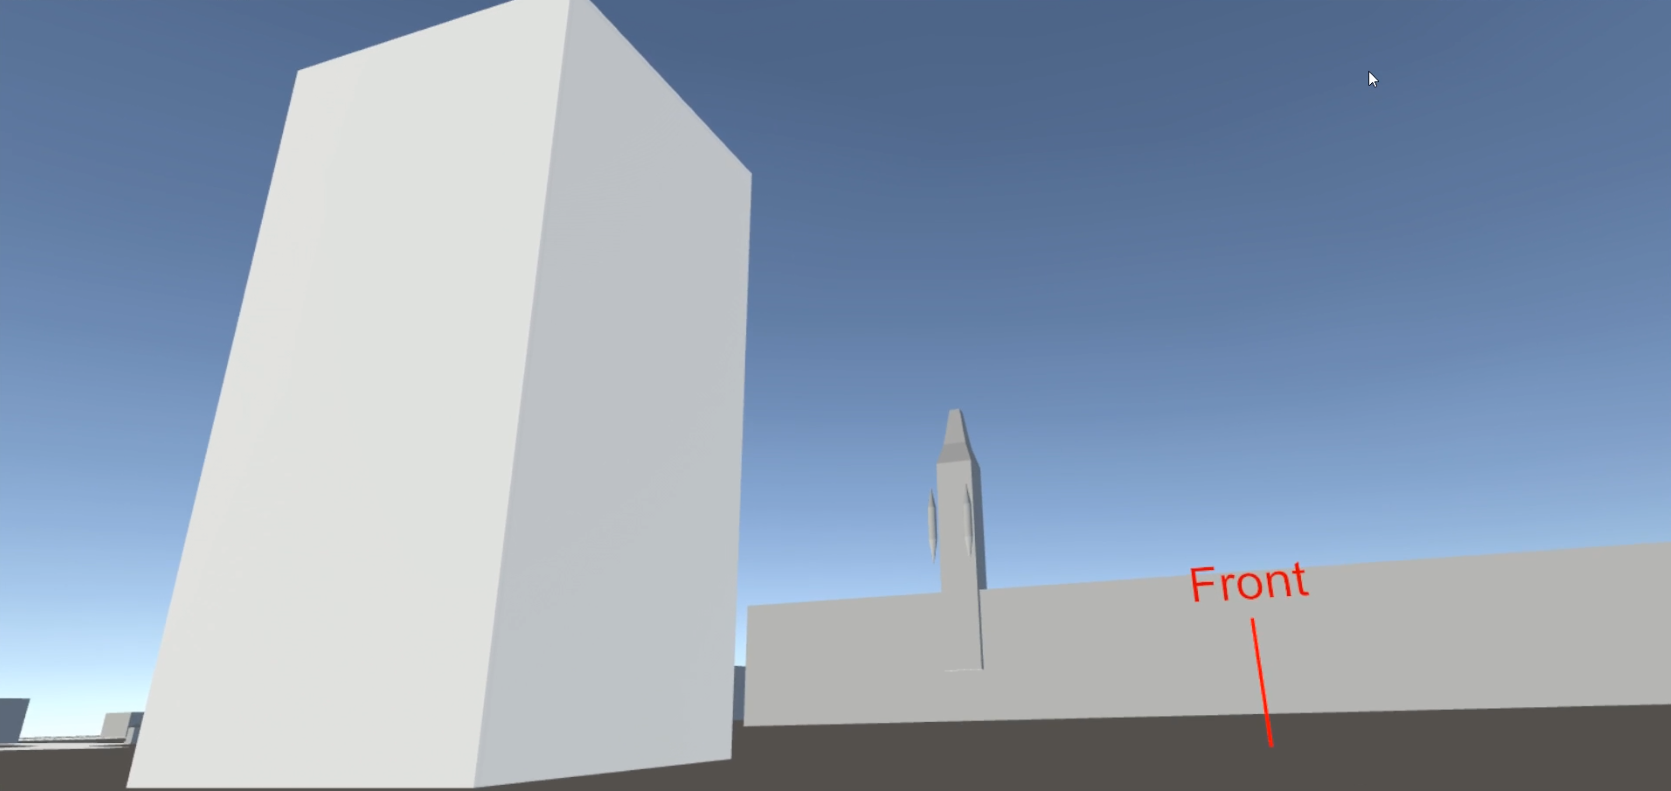
\includegraphics[width=0.7\linewidth]{figures/pilot2_environment_tutorial}}
	\par
	\subfloat[Experiment mode, the cylinder wall (front view)]{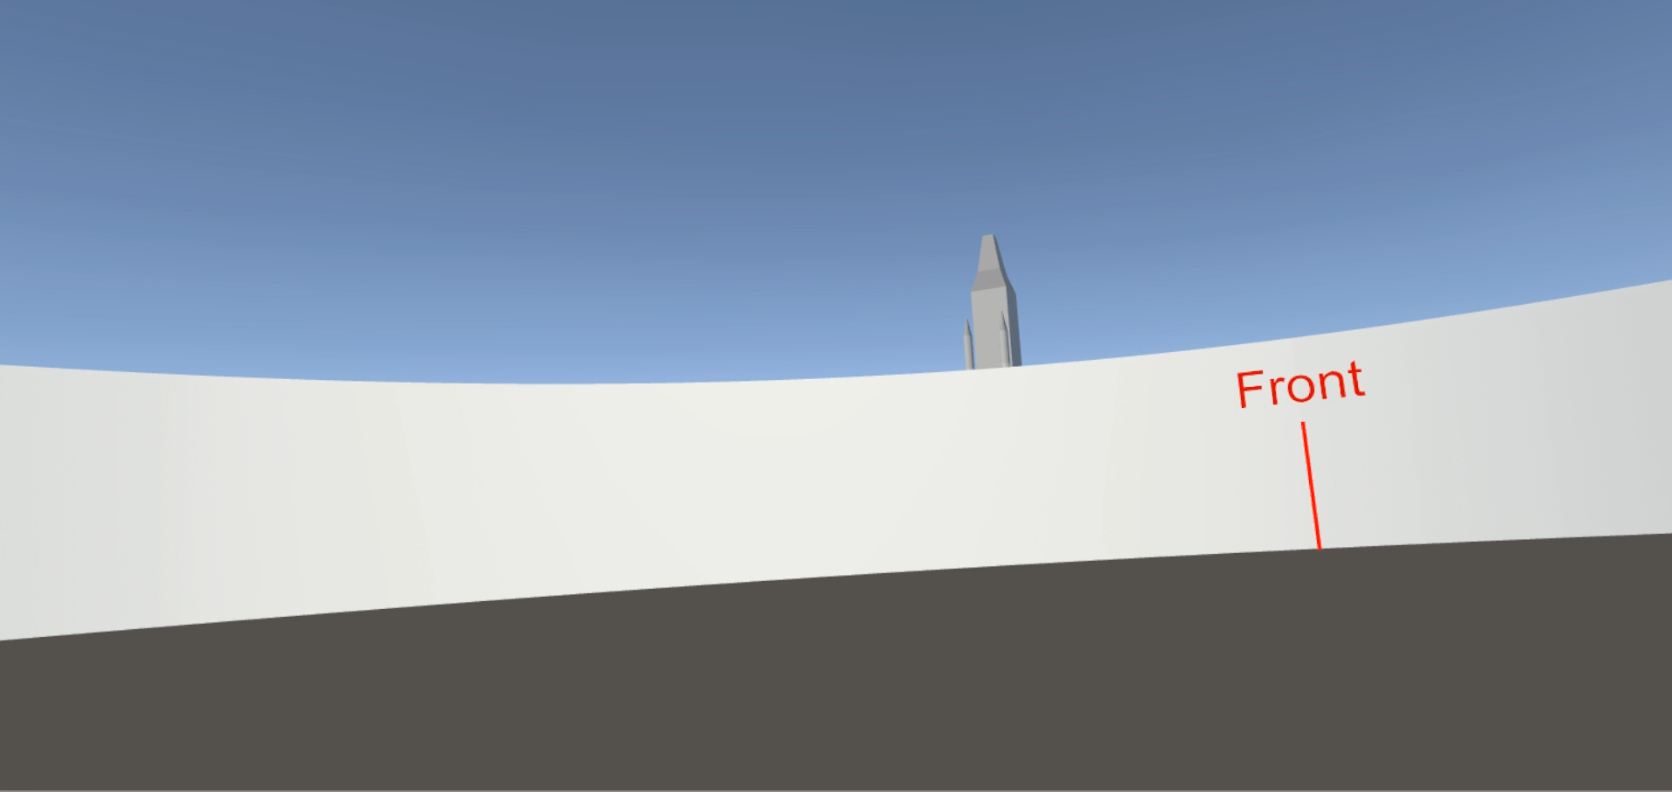
\includegraphics[width=0.7\linewidth]{figures/pilot2_tutorial_experiment_front}}
	\par
	\subfloat[Experiment mode, the cylinder wall ()back view)]{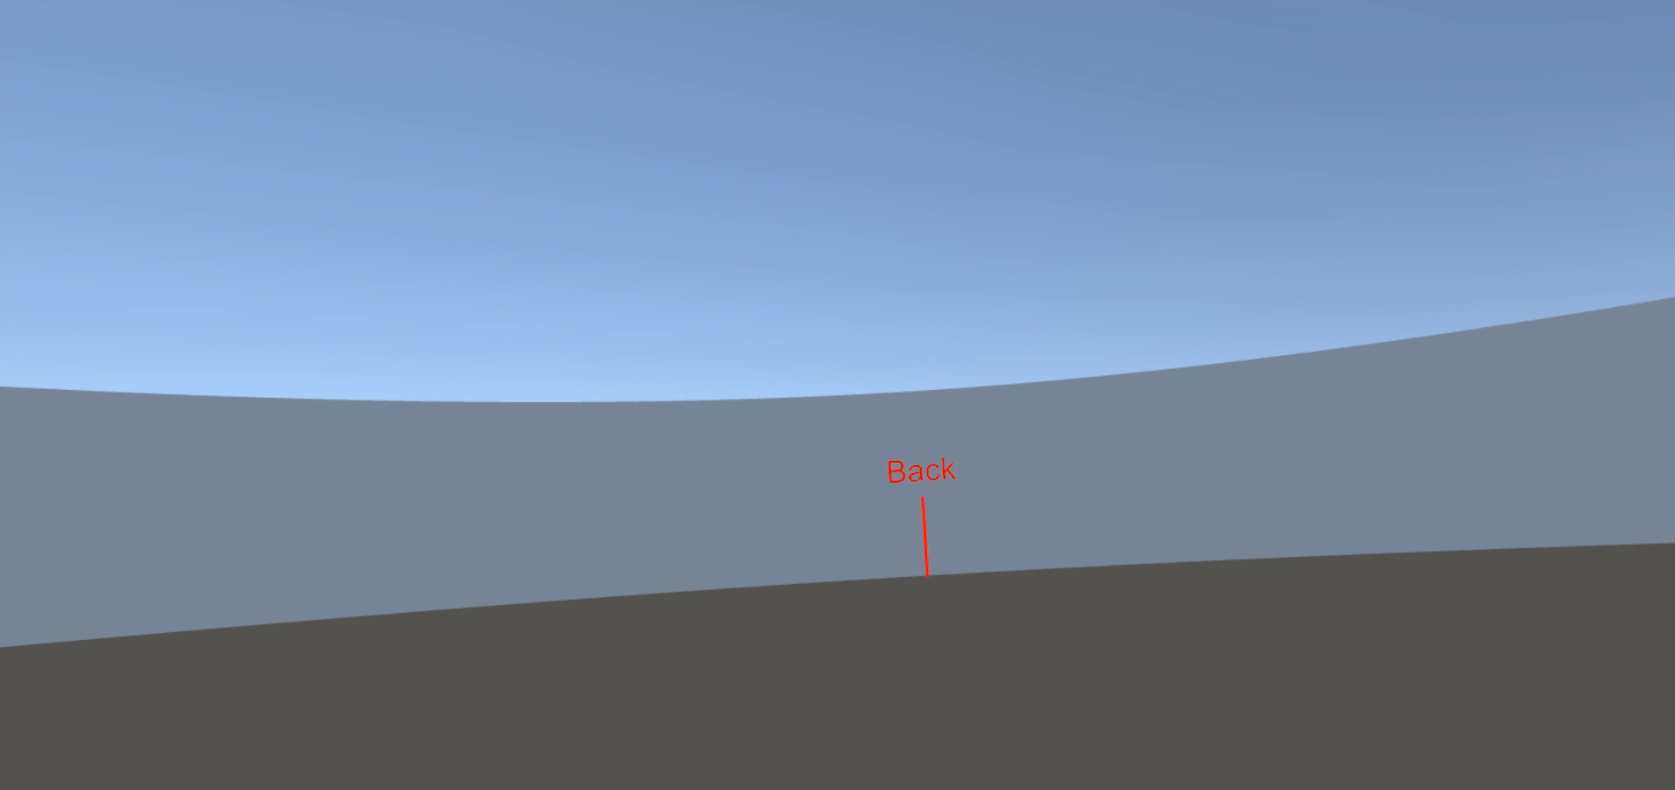
\includegraphics[width=0.7\linewidth]{figures/pilot2_tutorial_experiment_back}}
	\caption{Experiment environment}
	\label{fig:pilot2experiement_environment}
\end{figure}

% TODO: the participant, a participant, participant, participants?
The goal of the tutorial mode was to allow the participant to understand the correlation between the visually perceived movements of the building and the sound emitted. The affordances of the environment were explained prior to the tutorial.

In the tutorial mode, the building was visible, and the wall - invisible.
40 translations were pre-scripted for the actual experiment, 20 of which were demonstrated. The control panel for this experiment can be viewed in Fig. \ref{fig:pilot2tutorialcontrolpanelhighlighted}, the buttons that are highlighted in blue were used to initiate tutorial translations. These translations were initiated in the same order for all the participants, they are additionally visualized in Fig. \ref{fig:pilot2endpointstutorialtranlstaions}.

Participants were briefed to face the "Front" direction, when the experimenter voiced the path that the building was going to travel, or (in the experiment mode) the fact that a translation is about to get initiated. After that participants were allowed to move their head. This and the choice of the translation paths for the tutorial was informed by the idea of allowing the participant to build a complete picture, of how a translating building sounds in all the directions around the user. "Front" and "Back" directions were identified with text on a pole, and were always visible (Fig. \ref{fig:pilot2experiement_environment}).

\begin{figure}
	\centering
	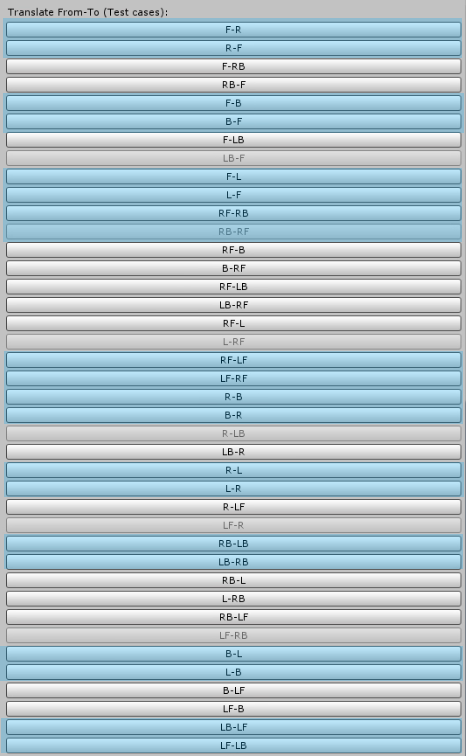
\includegraphics[width=0.7\linewidth]{figures/pilot2_tutorial_control_panel_highlighted}
	\caption{Control panel}
	\label{fig:pilot2tutorialcontrolpanelhighlighted}
\end{figure}

\begin{figure}
	\centering
	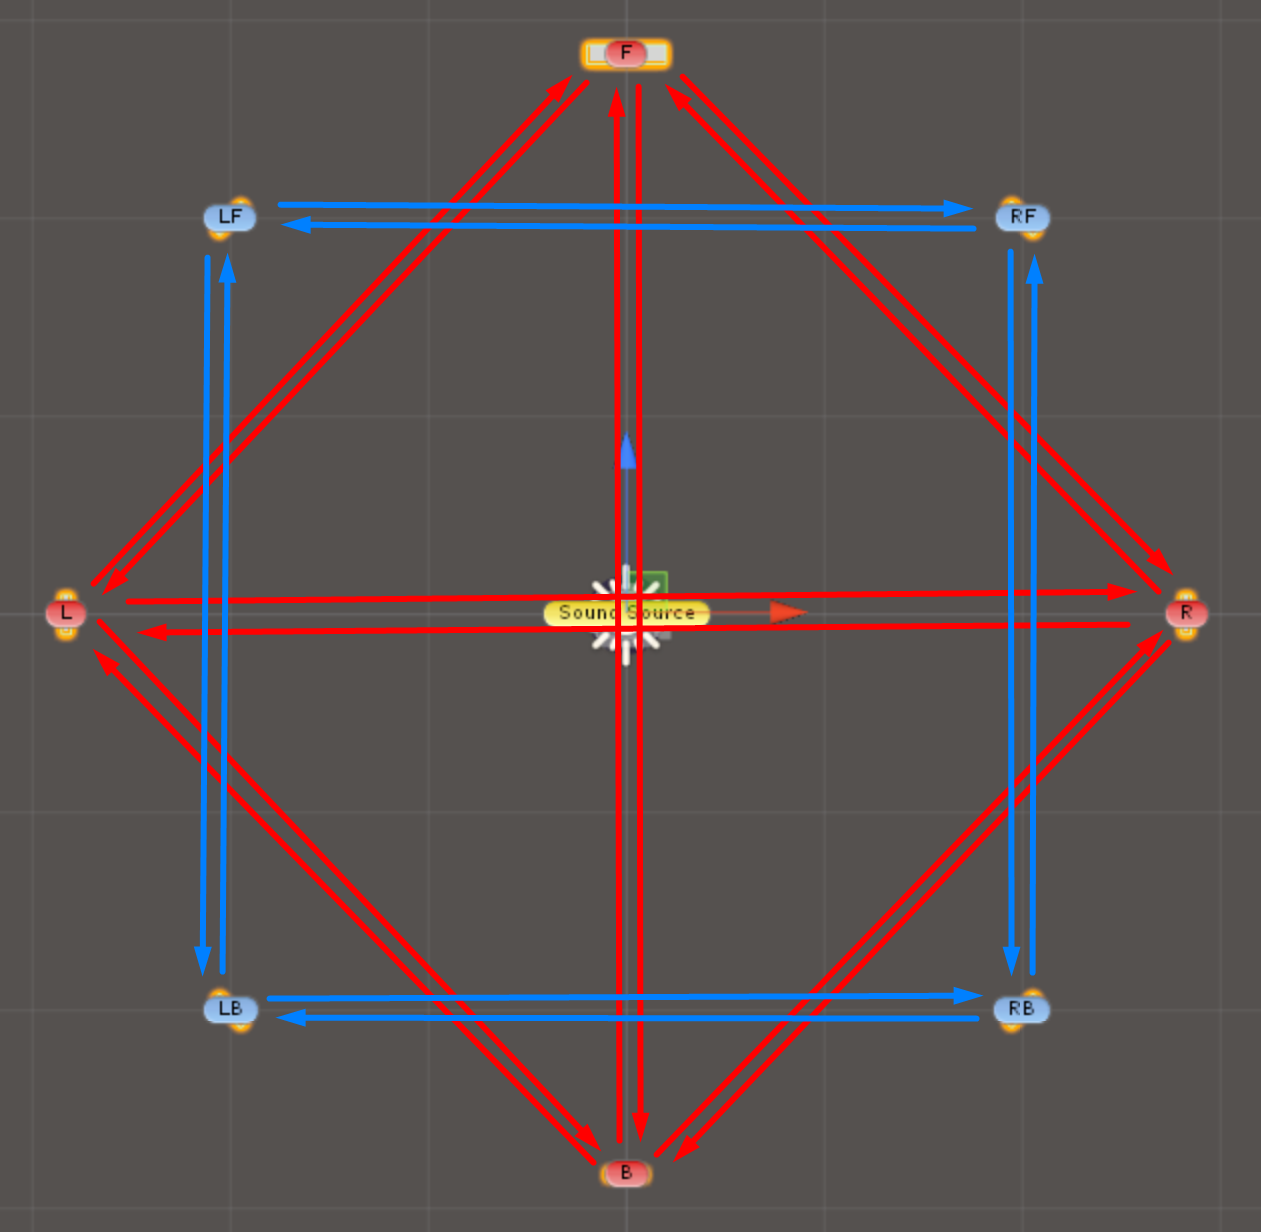
\includegraphics[width=0.7\linewidth]{pilot2_endpoints_tutorial_tranlstaions}
	\caption{Tutorial translations}
	\label{fig:pilot2endpointstutorialtranlstaions}
\end{figure}



After the tutorial translations were demonstrated, participants were asked if they were ready to proceed to the actual experiment. Only one participant asked to repeat some of the translations to gain a better spatial understanding.

In the experiment mode participants were not able to see the building, but would still hear the sounds when it started moving. The wall around the user was visible. The end-points of the translations of the building were always on this wall. Participants were asked to indicate where the building translated from and to with the help of a simulated laser pointer attached to the controller. The details of the controls can be found in Appendix \ref{app:pilot2_controls}.

All 40 translations were initiated in a pseudo-random order for each participant. This order was decided by the experimenter. Each translation could be initiated only once, to make sure no translations were initiated multiple times (after the initiation the button for this translation would be grayed-out and rendered inactive, see Fir. \ref{fig:pilot2tutorialcontrolpanelhighlighted}). The experimenter was responsible for  initiating the translations.
Participants answers were recorded by the system in a CSV file.

When participants went through all the 40 translations, the experiment would end. Experimenter thanked the participants and ask for their feedback concerning the experiment.

%\paragraph{Apparatus} The same, as in \ref{study_one} \nameref{study_one}, with addition of 6 \gls{dof} tracked controllers.

\paragraph{Study design}
This study used the repeated measures design with one independent variable - translation paths (40 values).
The building could travel between the total of 8 endpoints. These were moved equidistantly and  placed around the participant (approx. 28.3m away) along the cylinder wall (Fig. \ref{fig:pilot2endpoints}).
The auditory icon of a concrete bock sliding on a concrete surface from the previous experiment was used. The translation speed of the building was 30m/s.

\begin{figure}
	\centering
	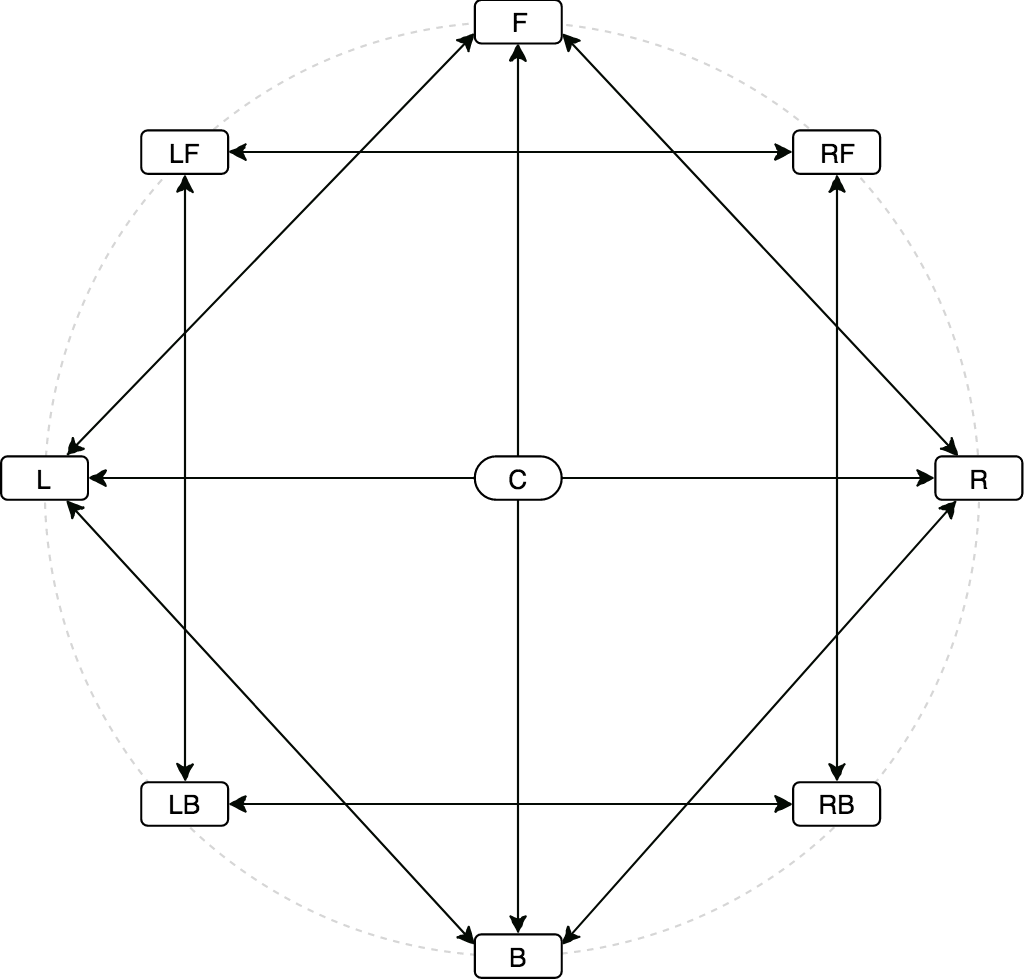
\includegraphics[width=0.7\linewidth]{figures/pilot2_endpoints}
	\caption{Translation endpoints}
	\label{fig:pilot2endpoints}
\end{figure}

\paragraph{Results}

A sample of the collected data can be seen in Fig. \ref{fig:pilot2datasample}. The link to the complete data can be found in Appendix \ref{app:pilot2data_collected}.

The following data was collected:
\begin{itemize}
	\item From X, From Y, From Z - start-point of the translation;
	\item To X, To Y, To Z - end-point of the translation;
	\item From Abbreviation, To Abbreviation - name abbreviation of the start- and end-points (i.e. "LB" corresponds to "Left Back");
	\item Translation Start, Translation Finish - time in seconds since the beginning of the game, until the translation started and finished, respectively;
	\item Guess From X, Guess From Y, Guess From Z - participant-perceived start-point of the translation;
	\item Guess To X, Guess To Y, Guess To Z - participant-perceived end-point of the translation;
	\item Guess Start, Guess Finish - time in seconds since the beginning of the game, until the participant indicated the start- and end-points of the translation;
	\item Angle From, Angle To - angle between the C-F (the line between the Center point and the Front point) and C-(From X, 0, From Z), C-(To X, 0, To Z), respectively;
	\item Guess Angle From, Guess Angle To - angle between the C-F and C-(Guess From X, 0, Guess From Z), C-(Guess To X, 0, Guess To Z), respectively;
	\item Divergence Angle From, Divergence Angle To - angular distance between the Angle From and Guess Angle From, Angle To and Guess Angle To, respectively.
\end{itemize}

\begin{figure}
	\centering
	\subfloat{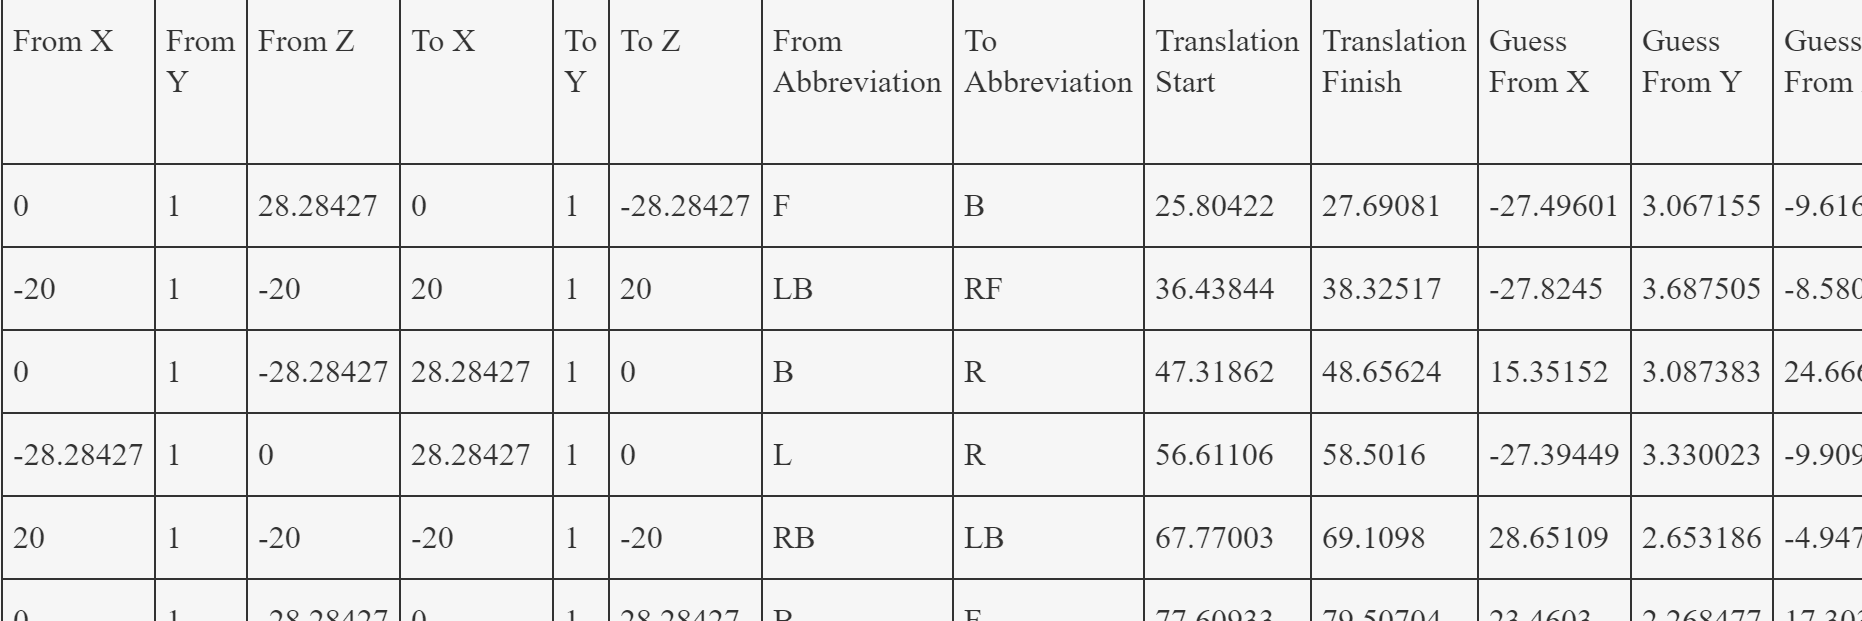
\includegraphics[width=0.7\linewidth]{figures/pilot2_datasample1}}
	\par
	\subfloat{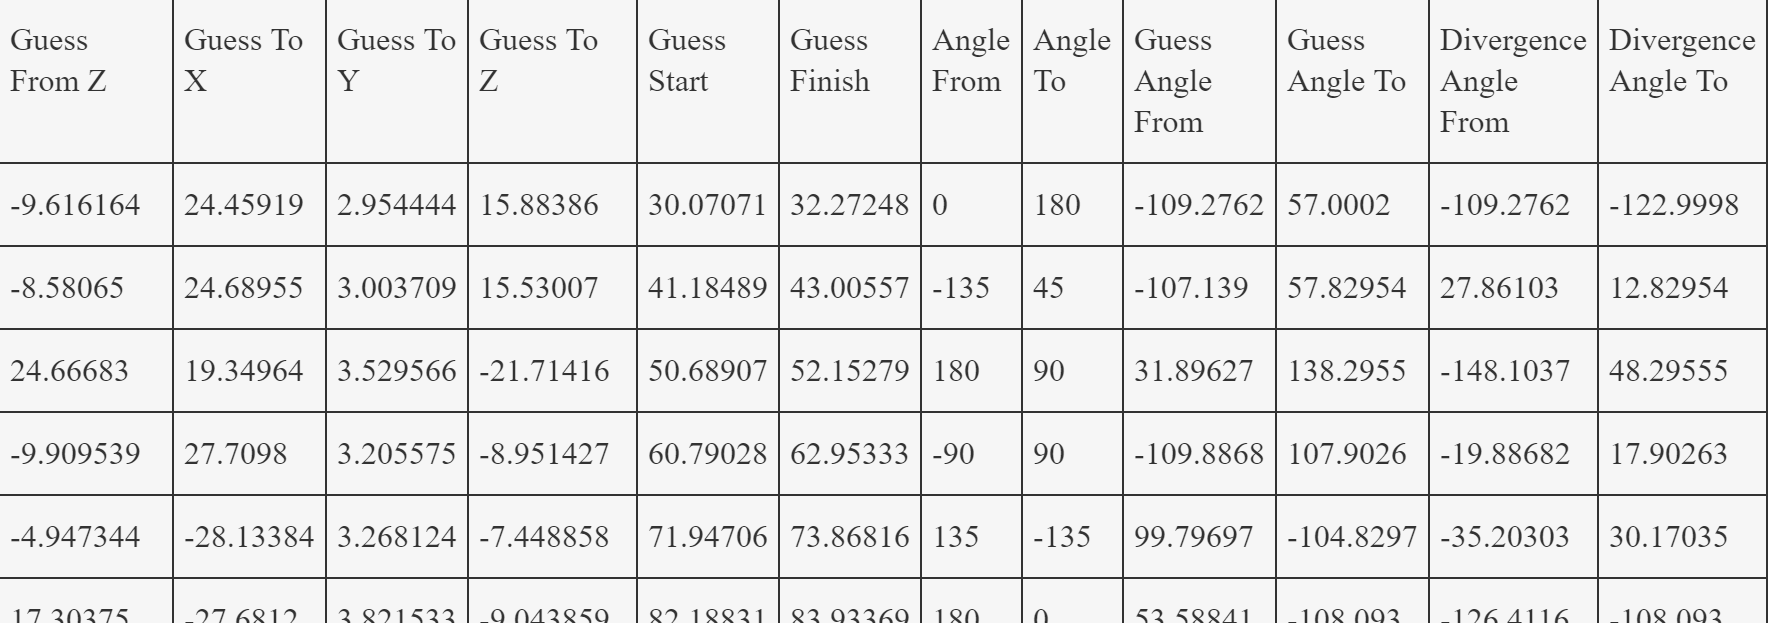
\includegraphics[width=0.7\linewidth]{figures/pilot2_datasample2}}
	\caption{Collected data sample}
	\label{fig:pilot2datasample}
\end{figure}



% Post-questionnaire summary
At least half of the participants reported having trouble to differentiate front and back translations. Some thought the building was always in the back, but decided to give some answers in-front just to balance the results. One participant indicated that everything was "easy and logical" when the building was visible, and unclear when it was not.

\paragraph{Discussion}
% Example visual result w/ explanation
The results of the experiment were represented visually, as seen in the Fig. \ref{fig:b-f}. One visualization was created for each out of 40 paths that the building traveled in the experiment (40 visualizations). These can be found in Appendix \ref{app:pilot2visual_analysis}.

\begin{figure}
	\centering
	\includegraphics[width=0.7\linewidth]{../Studies/SpatialJudgements/Generated/B-F}
	\caption{Example visualization of data for the translation path Back to Front}
	\label{fig:b-f}
\end{figure}

This visualization can be thought of as a top-down projection of the experiment environment.
Individual answers are shown with semi-transparent directional rays of red-blue gradient. The beginning of individual rays is wider and red, the ending - thiner and blue. The transparency value $t$ was approx. equal $7.7$, and was computed as $t = 100 / n_{p}$, where $ n_{p} $ is the number of participants.
The information in the left corner ("PATH") describes the actual translation path: "abbr." - name abbreviation of the path, "act." - actual angles the building traveled from and to. This data is also visualized with the green line, whose end-points are marked with big green circles and "From", and "To" labels.
The information in the right corner ("STATS (deg.)") gives the statistical data for this path in degrees: "mean" - mean values for the "Guess From" and "Guess To" entries, respectively. This information is also visualized with the red line, whose end-points are marked with small red circles and "m.From", and "m.To" (which stand for: "mean From" and "mean To", respectively).
Start- end end-points of translations are marked with their respective name abbreviations and deviation angles from the Front direction.

On this example we see the visualization of the guesses made by participants when the building traveled from Back to Front (B-F). A certain number of participants have guessed correctly, which is indicated by a brighter (or less transparent) overlay of the directional rays. The mean value goes from approx. $152.3\degree$ to approx. $- 30.8\degree$. The error of $\pm 45\degree$ can be considered negligible due to the limitations of the stereo headphones and the absence of the visual cues. At least 5 participants have guessed incorrectly, and at least one thought that the building moved from Front to Back, which is indicated by the red ray ending starting at the F point and going straight down.


% Interpretation of the results
The mean values for 29 out of 40 translations were close to the actual translation paths, if we assume the result being in the range of the negligible error of $\pm 45\degree$ as close. % Green dot
Among the other 11 translations, six could be considered close, if we eliminate the front-to-back confusion by mirroring either one, or both the mean start and mean finish endpoints along the imaginary L-R line.
% TODO: pic of this mirroring
% Mean deviation for deviation of start and end /points // <- estimate - apparently, not useful for the stats analysis: https://en.wikipedia.org/wiki/Unbiased_estimation_of_standard_deviation

% Conclusion
Regardless, of many erroneous guesses, the analysis shows promise for the given setup, and, considering the previous success of \cite{gutwin_chalk_2011} in representing spatial information with audio feedback through the stereo headphones, as well as the fact that in the final study participants will have visual cues to aid them in finding the sound source, and the fact that they won't be forced to always face the same direction, this approach deserves a further analysis.

%\subparagraph{Limitations}

% Number of participants














\section{Workspace Awareness in Immersive Virtual Reality}
\label{final_study}
% TODO: use the term "feedthrough" somewhere in the experiment description

% Goal of the study
The goal of this study was to analyze \gls{wa} that participants have of others present in the same immersive \gls{vr} environment. Participants were presented with a primary and secondary tasks. Primary task was tracing 3D models with a 3D brush, and secondary task was a \gls{wa} task - reporting changes to the environment.
%\paragraph{Methods}
The evaluated aspects of \gls{wa} were participants’ reaction speed when provided with different types of awareness presentation : sonification (audio feedback) and/or visualization (via the minimap) of the buildings' movement.

\paragraph{Participants}
12 participants (8 men and 4 women) were recruited among friends, employees from the chair, and students from the \gls{tum}; ages ranged from 22 to 32 (mean 25.2, std. 2.5). Only one participant reported having "partially" good hearing, others reported good hearing. 3 people reported to be familiar with \gls{vr} technology, among them, one person reported being a proficient gamer and one - having partaken in driving simulator studies. Participants were a mix of gamers, non-gamers, and casual gamers. Participants were also equally distributed among people who had experience with \gls{vr}, those who had some experience, and those who had no prior experience. Two reported being online gamers, and another two - occasional online gamers. Only one person had prior experience with architecture, and had worked in the field. One participant tried 3D drawing in the system before, but otherwise none had seen the system before, or took part in the previous studies.

\paragraph{Procedure}
Participants were given a written and verbal introduction to the experiment,
and were asked to sign the consent form for using their data.
Next, they were placed in the immersive \gls{vr} environment, which implemented 2 modes: tutorial and experiment (Fig \ref{fig:finalstudy_immersive_vr_environment}). In the tutorial mode, only one building (the clock tower) and the test tracing shape would be visible.
Participants learned how to use the 3D voxel brush for tracing the shapes (Fig. \ref{fig:finalstudyvoxeldrawing}), the laser pointer to indicate they noticed changes to the environment, and the minimap to locate the moving buildings. Following that, the audio feedback was introduced, and the differences between the tutorial and the actual experiment part were explained. Participants went through a small scenario, resembling the experiment, where they were asked to trace a pillar, and in the meanwhile try to catch the moving building a couple of times. They were also asked to keep track of how the building sounds and where it is visually.

\begin{figure}
	\centering
	
	\subfloat[Tutorial environment, the clock tower]{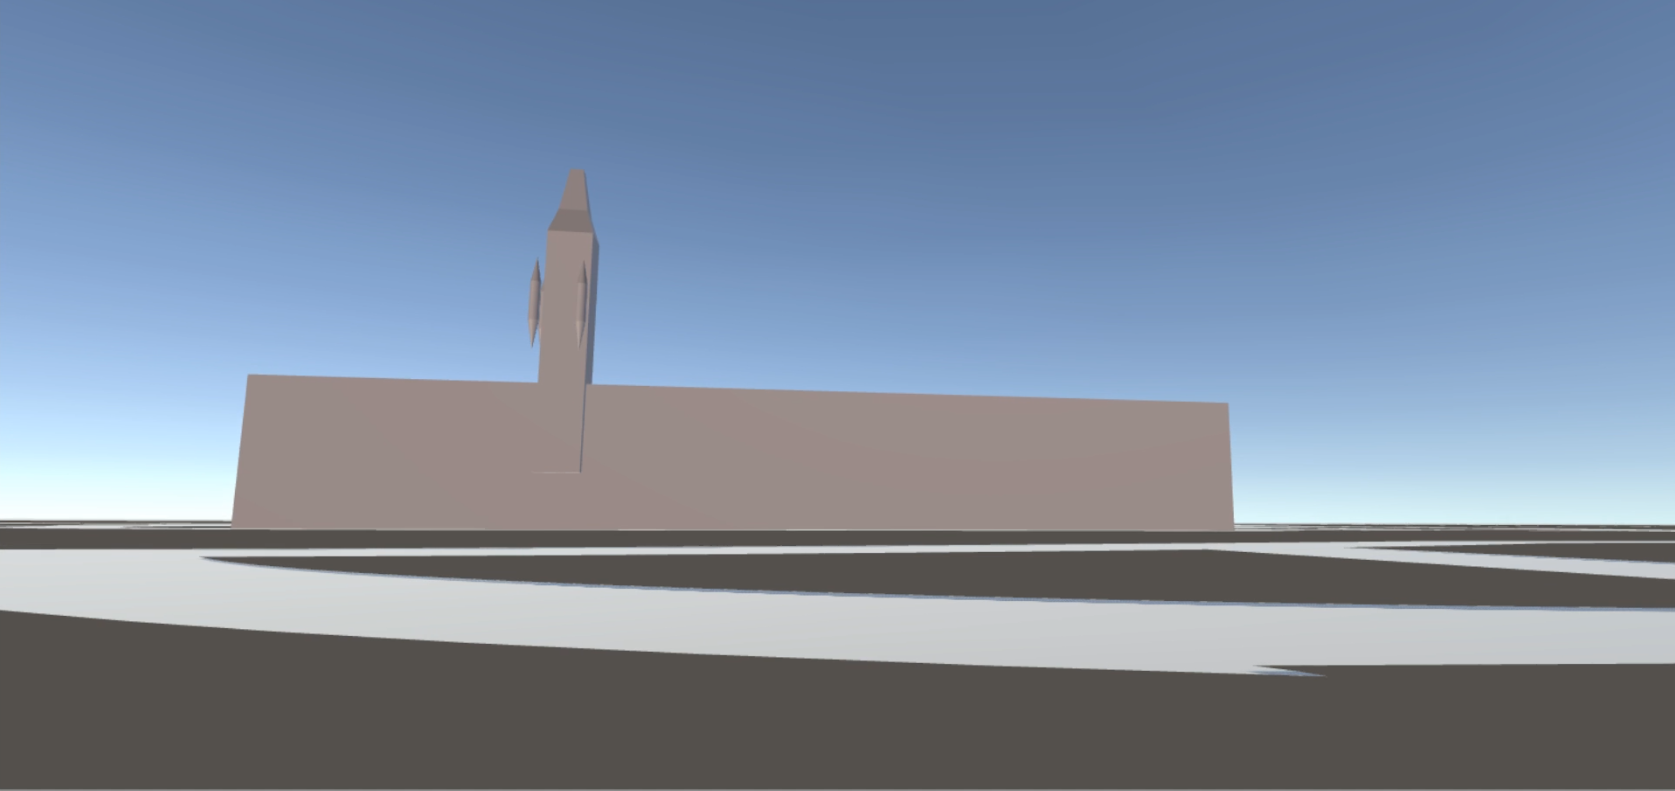
\includegraphics[scale=.29]{D://Documents/studies/ss18/Thesis/tum-thesis-latex/figures/finalstudy_environment_tutorial}}
	\par
	\subfloat[Experiemnt environment, the clock tower]{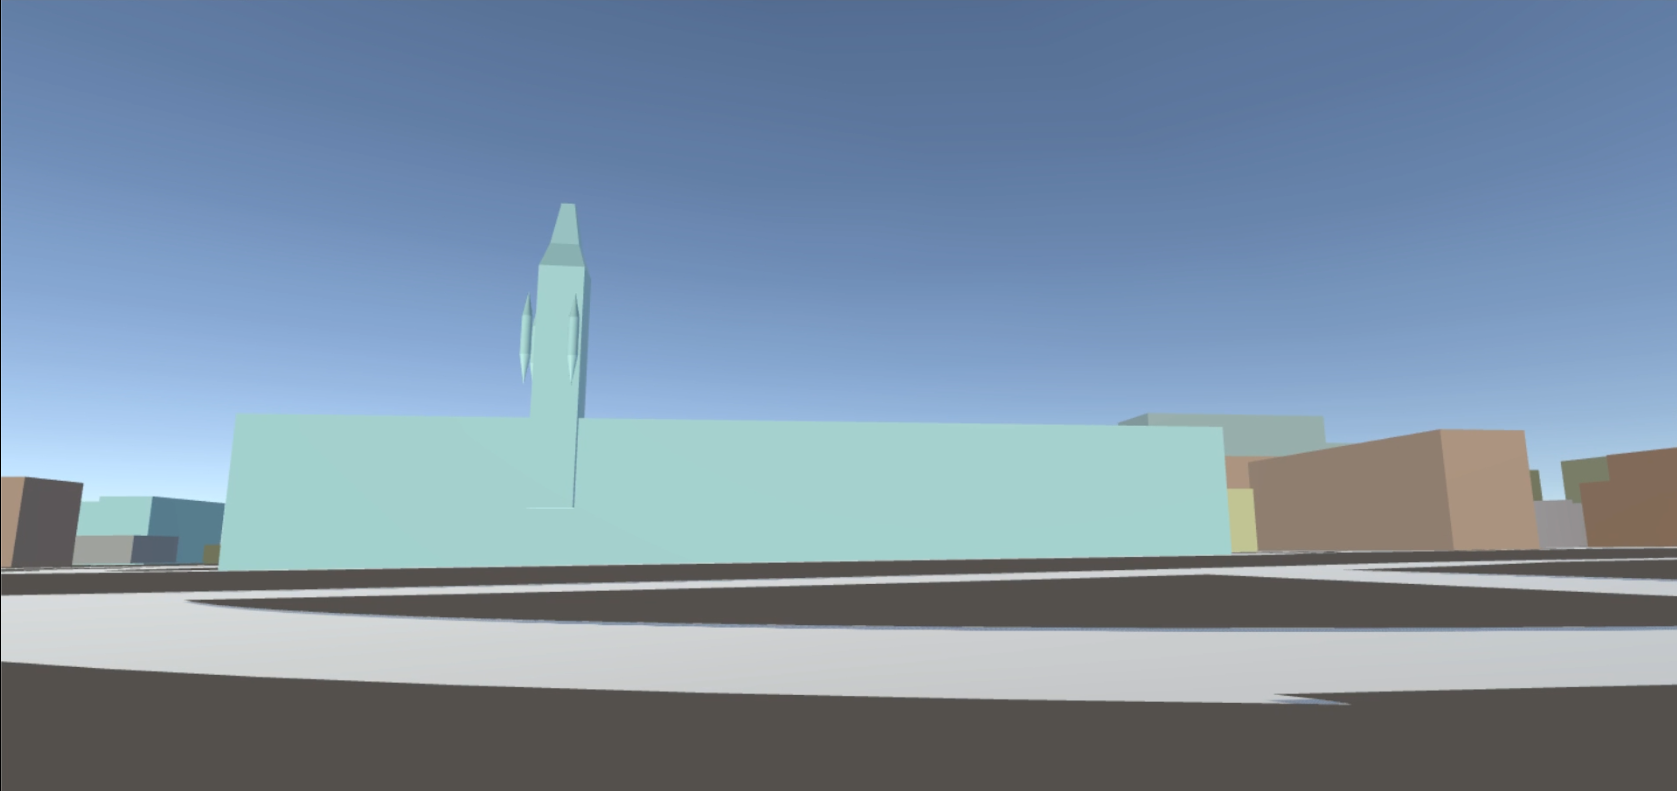
\includegraphics[scale=.29]{D://Documents/studies/ss18/Thesis/tum-thesis-latex/figures/finalstudy_environment2}}
	\par
	\subfloat[Experiemnt environment, the tracing shape]{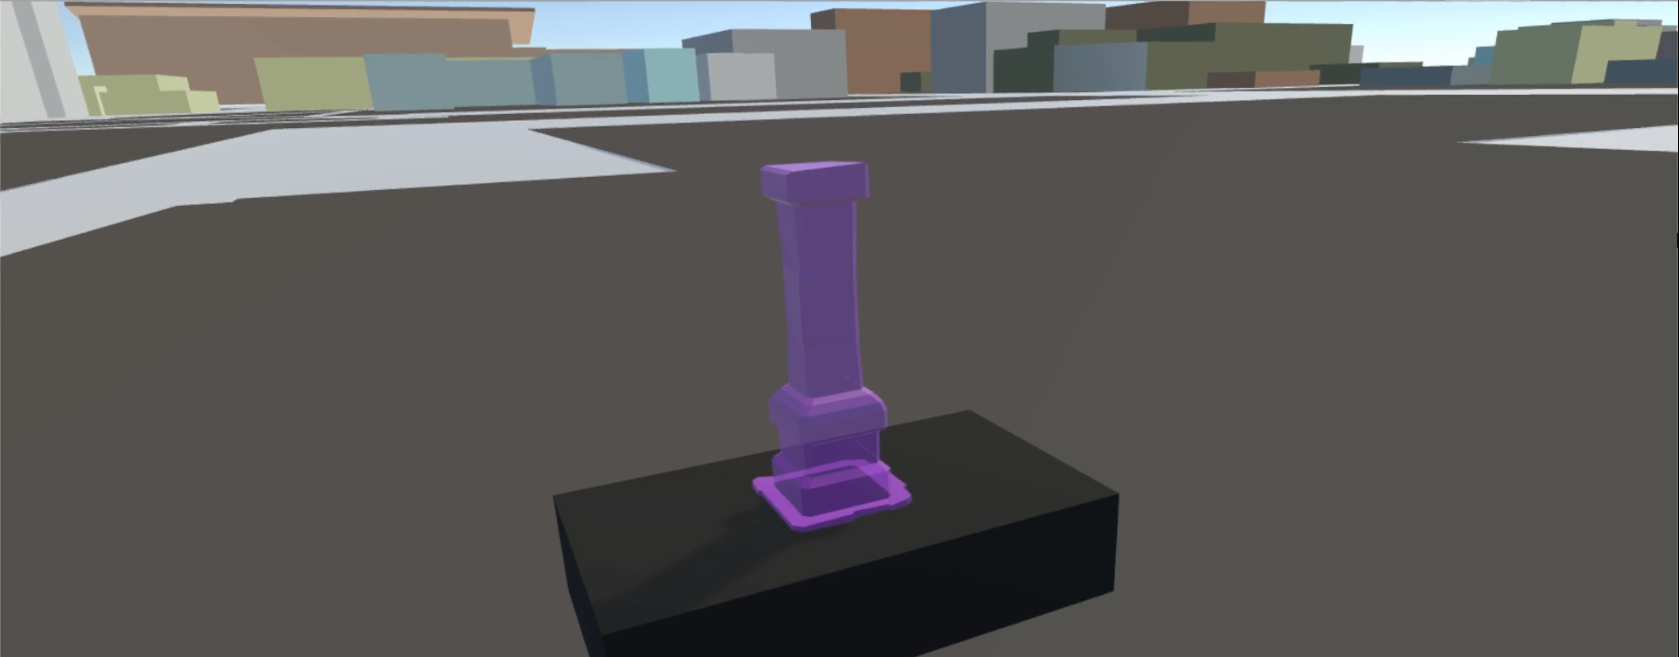
\includegraphics[scale=.29]{D://Documents/studies/ss18/Thesis/tum-thesis-latex/figures/finalstudy_environment}}
	
	\caption{Virtual environment}
	\label{fig:finalstudy_immersive_vr_environment}
\end{figure}

\begin{figure}
	\centering

	\subfloat[Tracing shape]{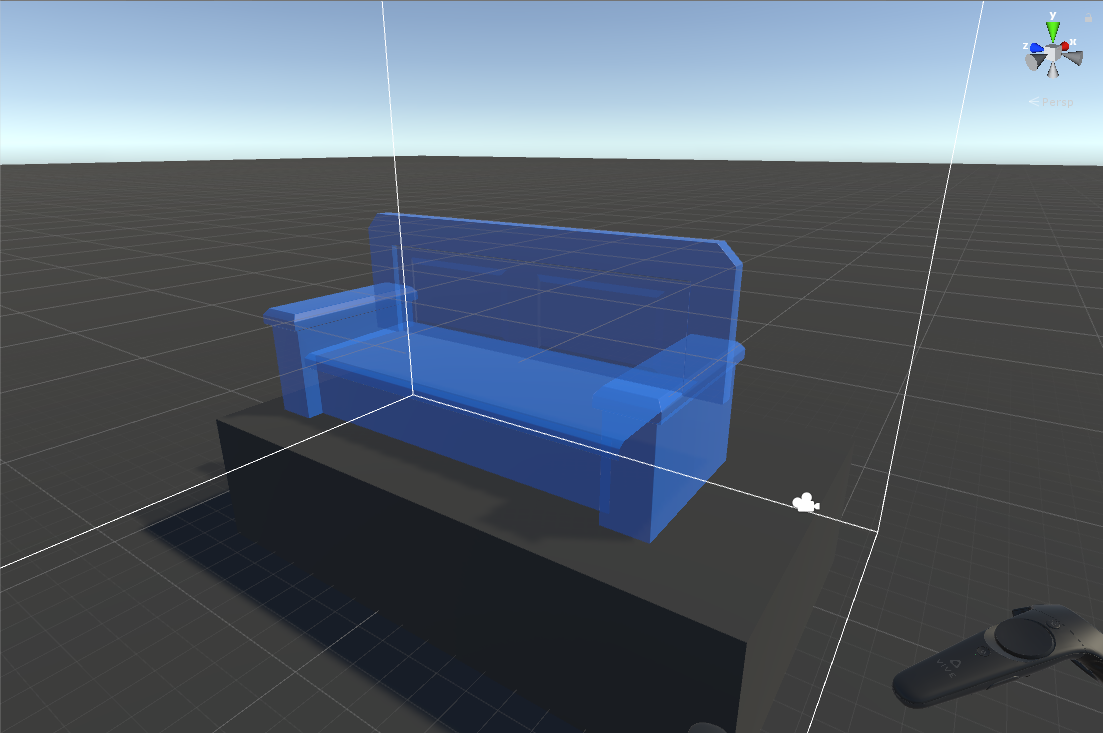
\includegraphics[width=0.7\linewidth]{figures/finalstudy_voxeldrawing1}}
	\par
	\subfloat[Partially traced shape]{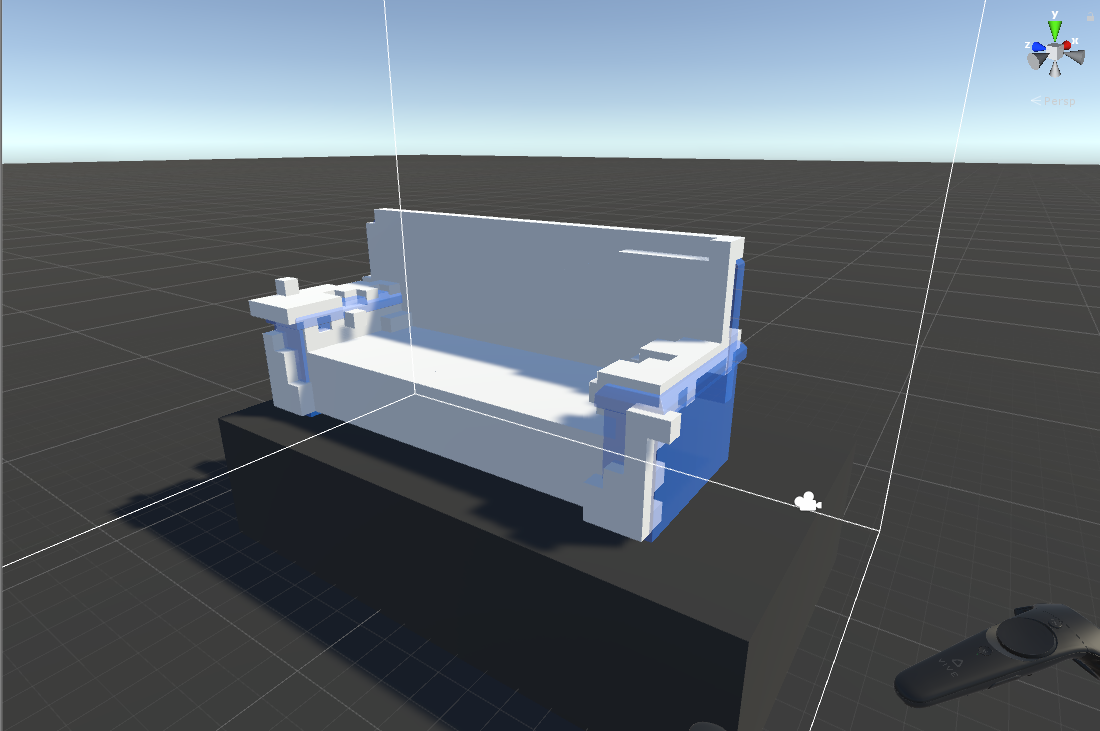
\includegraphics[width=0.7\linewidth]{figures/finalstudy_voxeldrawing2}}
	\par
	\subfloat[Tracing shape and voxel drawing side-by-side]{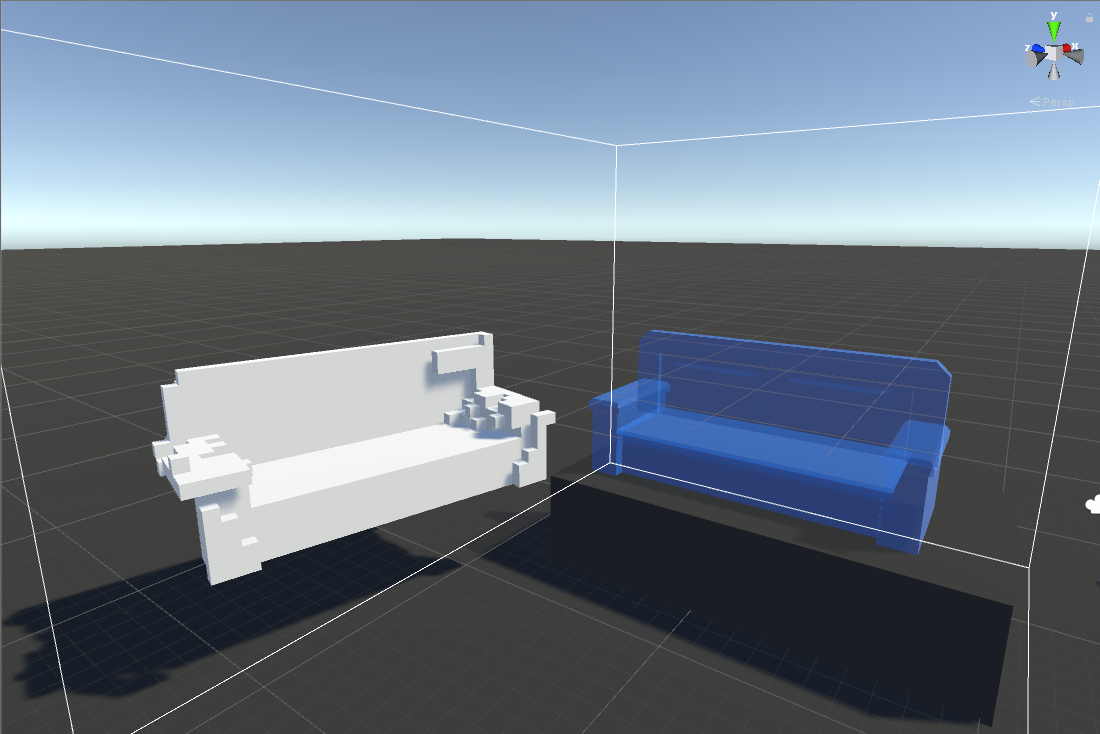
\includegraphics[width=0.7\linewidth]{figures/finalstudy_voxeldrawing3}}

	\caption{Voxel drawing}
	\label{fig:finalstudyvoxeldrawing}
\end{figure}


During the actual experiment, each participant was tested in each of the 3 test groups: \textit{Minimap and Sound}, \textit{Sound Only}, and \textit{Minimap Only}. Participants were instructed to keep focus on their main task and treat the experiment not as a test of their abilities to notice all the moving buildings, but rather as a test to check how good the system was in informing them of these changes. 
When participants were done with a shape, they would voice this to the experimenter, and he would save the current voxel drawing, and switch the tracing shape to the next one.
At the end of the experiment, participants were asked to fill in a self-report questionnaire.
Participants did not rest between the different conditions. 
After the end of the experiment, participants were asked to fill out a questionnaire (Appendix \ref{app:final_study_questionnaire}).

\paragraph{Task}
Participants were asked to follow a scenario, in which there were two architects (A1 and A2), who performed their individual domain tasks in an urban district (\ref{fig:urbandistrict}) in \gls{vr}. A1 (participant) had two tasks, primary and secondary. The primary task was to trace given 3D shapes with a 3D voxel brush, which was implemented for one of the tracked 6-\gls{dof} controllers. Meanwhile, A2 (simulated invisible agent) could translate any building in the district to any other part of the district at any time. The secondary (workspace awareness) task of A1 was to keep track of changes to the environment and point them out with a virtual laser pointer (another tracked 6-\gls{dof} controller). The details of controls can be found in Appendix \ref{app:finalstudy_controls}

\begin{figure}
	\centering
	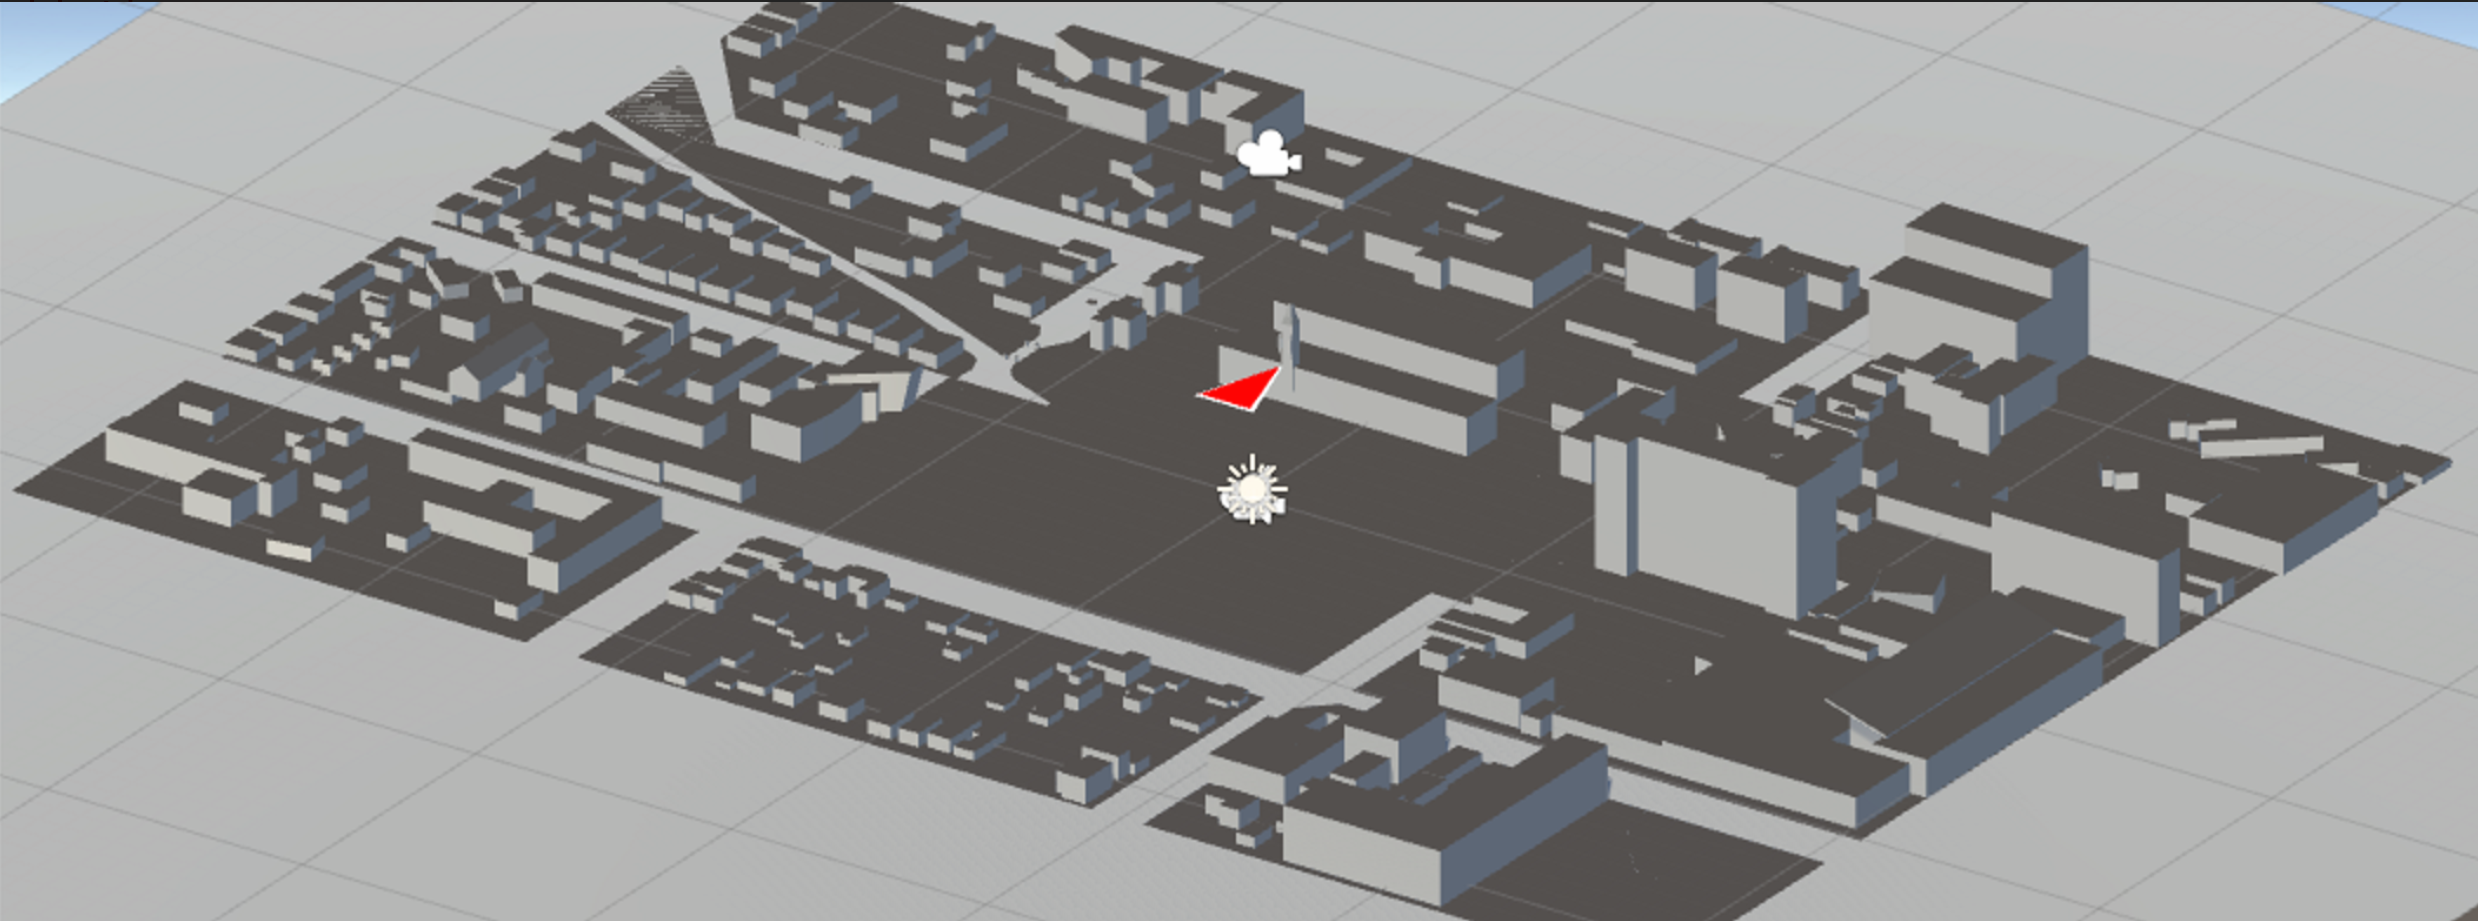
\includegraphics[width=0.7\linewidth]{figures/urban_district}
	\caption{Simulated urban district for the \gls{wa} study}
	\label{fig:urbandistrict}
\end{figure}


%\paragraph{Apparatus} The same, as in \ref{study_two} \nameref{study_two}.

% Study Factors and Conditions: what my factors are, conditions == independent variables' values
% + Repeated-measures design?
\paragraph{Study design}
%\textit{Experimental Design} 
This study followed the repeated measures design with one independent variable - the type of awareness presentation. 3 controlled awareness presentations were used
\begin{itemize}
	\item minimap of the district (\ref{fig:minimap_controller});
	\item audio feedback emitted by translating buildings in the scene (sound of a concrete block sliding on a concrete surface);
	\item combination of the minimap and audio feedback.
\end{itemize}

Awareness presentations were rotated for each participant, so that each presentation was seen in the same position equal number of times. 
Each awareness presentation was tested for ten minutes, during which exactly eight buildings were randomly chosen and translated. In total, 24 data points were measured per participant in each session. Data collected were the reaction speed in determining the position of a moving building (catching it), along with 3D drawings created by participants. If the participant failed to catch the building, the reaction time was recorded as 0.
% TODO: add some of the voxel drawings here or to the appendix

\begin{figure}[h]
	\centering
	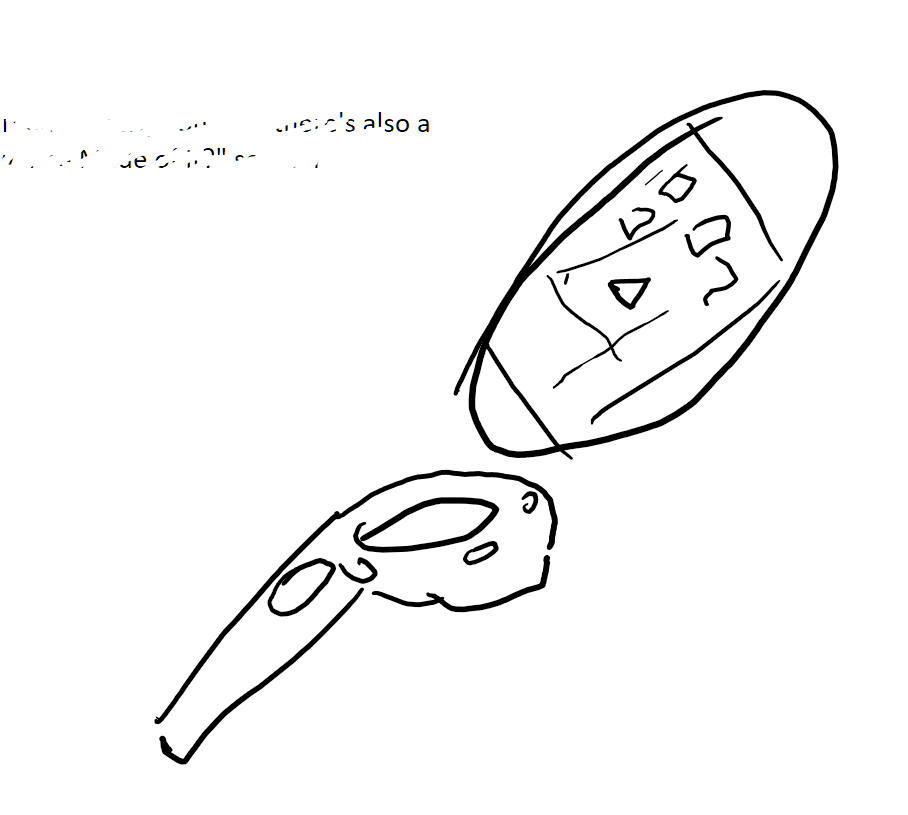
\includegraphics[width=0.7\linewidth]{figures/placeholders/minimap_controller}
	\caption{Controller with the minimap}
	\label{fig:minimap_controller}
\end{figure}

The total of 13 tracing shapes were prepared for the participants: 1 tutorial shape and 12 experiment shapes (Appendix \ref{app:finalstudy_tracingshapes}).
Participants went through them in the same order at the pace that they felt comfortable with.

\paragraph{Comparison with \nameref{par:shared_chalkboard_application}}
Since, this study extends upon \cite{gutwin_chalk_2011}, this paragraph provides the comparison of the two.
The main difference between - workspace is no longer a 2D plane, but an immersive 3D \gls{vr} environment. This means, first of all, that were able to look around the workspace, and notice changes to the environment, even without the help of the minimap or audio feedback. 
Second of all this 
% TODO: also, the fact that the head was tracked and this influenced the sound behaviour

Second distinction was in the primary task of the participant and the simulated agent. In \cite{gutwin_chalk_2011} the participant performed the same task, as an agent: drawing with chalk. Additionally, the participant's actions emit the same sound at a lower volume as the agent's actions. In this study, the primary task of the participant is - 3D drawing with voxels. This activity doesn't emit any sound. It is also different from the agent's task - translation of buildings in the urban district. Nevertheless, the tasks are still contextually related with regards to the architectural activity in urban environment.

In terms of the \gls{wa} framework, \cite{gutwin_chalk_2011} aim to answer the \textit{What?} and \textit{Where?} questions about the workspace: what is being done, and where is it being done. This study follows the same idea. In terms of \gls{sa}, just like \cite{gutwin_chalk_2011}, the present study touches on all 3 of its levels: 
\begin{enumerate}
	\item Perception: participant realizes that something is happening in the environment;
	\item Cognition: they understand that it is a building moving, and can locate;
	\item Projection: participant sees or hears the way that building is moving, and based on this, tries to catch it at its next position.
\end{enumerate}

\begin{comment}
\cite{gutwin_chalk_2011} do not specify the details of their spatial sound, however, since it was a 2D study, it is plausible that all sounds originate in the same plane, we will call it sound plane. In case of \cite{gutwin_chalk_2011} this plane could have been positioned in 3 different ways: vertically, horizontally, or somewhere in-between (Fig. \ref{fig:gutwinvsmystudysoundplane}a). In all cases, where the plane is positioned in an orientation that is different from the orientation of the screen, participants would have to build a mapping between for the interface. In this study, sounds are also emitted from the same plane, which is positioned horizontally (Fig. \ref{fig:gutwinvsmystudysoundplane}b).

Other similarities between the two studies include: the study design, the object of analysis (\gls{wa}), and the use of auditory icons for auditory feedback.

% TODO: re-draw: make a), b) subfloats
\begin{figure}[h]
	\centering
	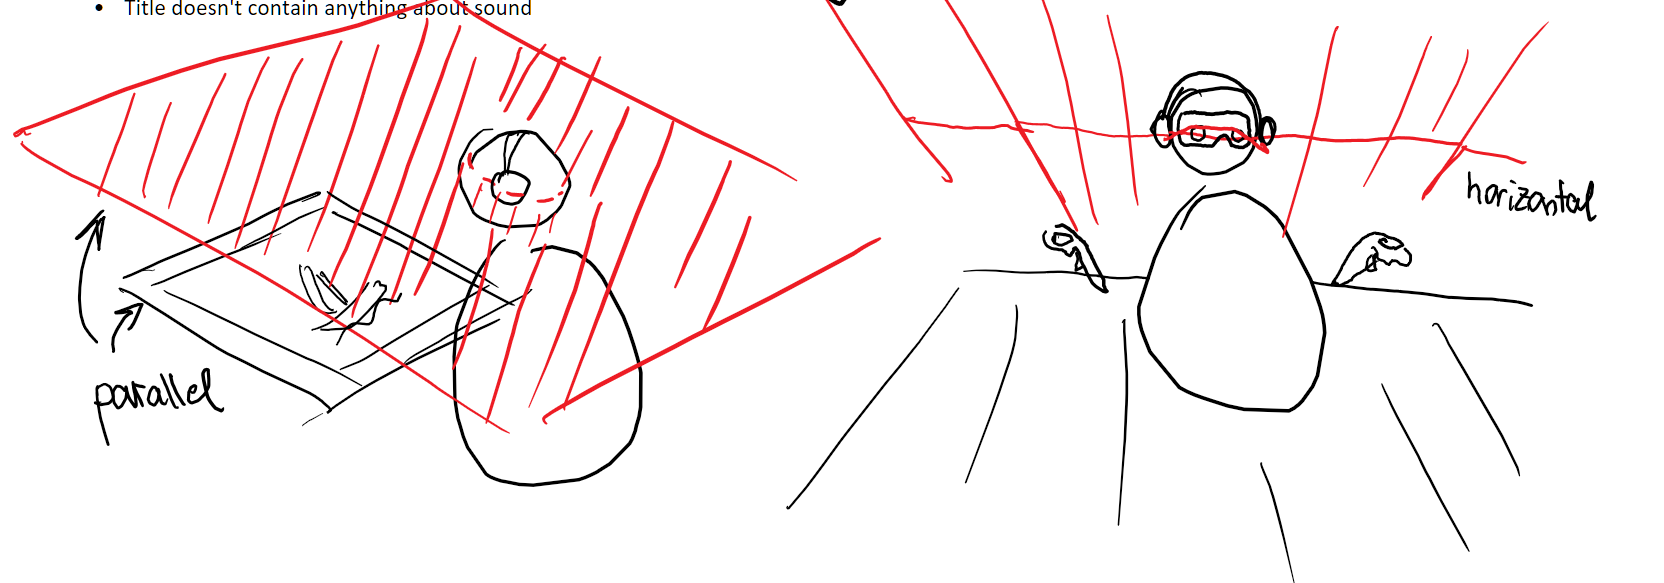
\includegraphics[width=0.7\linewidth]{figures/gutwin_vs_my_study_sound_plane}
	\caption{Comparison of sound emission planes}
	\label{fig:gutwinvsmystudysoundplane}
\end{figure}
\end{comment}

% TODO: linebreak
\begin{table}[h]
  \caption{Study comparison}
  \label{table:study_comp}
  \begin{tabularx}{\linewidth}{|X|X|X|}
  \hline
                             & \textbf{Shared chalkboard application study}                & \textbf{Workspace Awareness in Virtual Reality study}           \\ \hline
  \centering \textbf{Workspace dimensions}				 & 2D									   & 3D \\ \hline
  \centering \textbf{Participant's primary task} & The same as the primary for the simulated agent & Contextually related \\ \hline
  %\centering \textbf{Sound plane}      & Not specified             & Horizonatal          \\ \hline
  %\centering \textbf{Type of auditory cues}                 & Auditory icons        & Auditory icons       \\ \hline
  \centering \textbf{Object of analysis}         & Workspace awareness   & Workspace Awareness  \\ \hline
	\centering \textbf{Attentional demand}         & Variable difficulty of the tracing activity   & Variable difficulty of the tracing activity; shift of focus from the participant's personal evaluation to the system evaluation; personal motivation to see their 3D drawings \\ \hline
	  \centering \textbf{Radar size}         & Variable (small, medium, large)   & Constant (medium)  \\ \hline
	    \centering \textbf{Workspace clutter}         & Variable (none, sparse, dense)   & Constant (dense)  \\ \hline
	    \centering \textbf{Measurements collected}         & Accuracy in determining when, where, and what type of action occurred   & Accuracy in determining when and where the action occurred  \\ \hline
  \end{tabularx}
\end{table}

\paragraph{Results}
A sample of the collected data can be seen in Table  \ref{tab:finalstudy_datacollected}. Disambiguation of the colors can be found in the \textit{Issues and shortcomings }paragraph under \textit{Data collected}. The link to the complete data can be found in Appendix \ref{app:final_study_data_collected}.

The following was collected:
\begin{itemize}
	\item Translation id - unique ID number for the translation, which was constructed in the following way: yyyyMMddHHmmssffff (where "yyyy" is the year, "MM" is the month, and so on);
	\item Reaction time - time in seconds between the start of a random translation, until it was caught. If the translation was not noticed by the a participant, or they were not able to catch it, the assigned value is 0;
	\item Group - number code for different experiment groups: 1 - \textit{Minimap and Sound}, 2 - \textit{Sound Only}, 3 - \textit{Minimap Only}.
\end{itemize}

\begin{table}[]
	\centering
	\caption{Data collected for the 1-st user}
	\label{tab:finalstudy_datacollected}
	\begin{tabular}{|l|l|l|}
		\hline
		\textbf{Translation id} & \textbf{Reaction time} & \textbf{Group} \\ \hline
		201809141429023350      & 8.785538               & 1              \\ \hline
		201809141430303052      & 0                      & 1              \\ \hline
		201809141431203241      & 10.3826                & 1              \\ \hline
		201809141432414310      & 8.152039               & 1              \\ \hline
		201809141433516256      & 5.937988               & 1              \\ \hline
		201809141434408394      & 0                      & 1              \\ \hline
		201809141435519841      & 6.283508               & 1              \\ \hline
		\rowcolor[HTML]{FFCC67} 
		201809141436307651      & 6.861633               & 1              \\ \hline
		201809141439369338      & 7.19519                & 3              \\ \hline
		201809141440282911      & 7.336426               & 3              \\ \hline
		201809141441404922      & 11.57239               & 3              \\ \hline
		201809141443240140      & 9.522339               & 3              \\ \hline
		201809141444102440      & 8.072632               & 3              \\ \hline
		201809141445294328      & 5.132324               & 3              \\ \hline
		201809141446249932      & 5.532593               & 3              \\ \hline
		\rowcolor[HTML]{FFCC67} 
		201809141447016237      & 0                      & 3              \\ \hline
		\rowcolor[HTML]{FE0000} 
		201809141450017908      & 6.33374                & 2              \\ \hline
		201809141451396501      & 0                      & 2              \\ \hline
		201809141452332029      & 6.967896               & 2              \\ \hline
		201809141453432883      & 5.815063               & 2              \\ \hline
		201809141454292257      & 0                      & 2              \\ \hline
		201809141455206412      & 0                      & 2              \\ \hline
		201809141456128075      & 0                      & 2              \\ \hline
		201809141457263717      & 13.1925                & 2              \\ \hline
	\end{tabular}
\end{table}

\begin{comment}
\begin{figure}
	\centering
	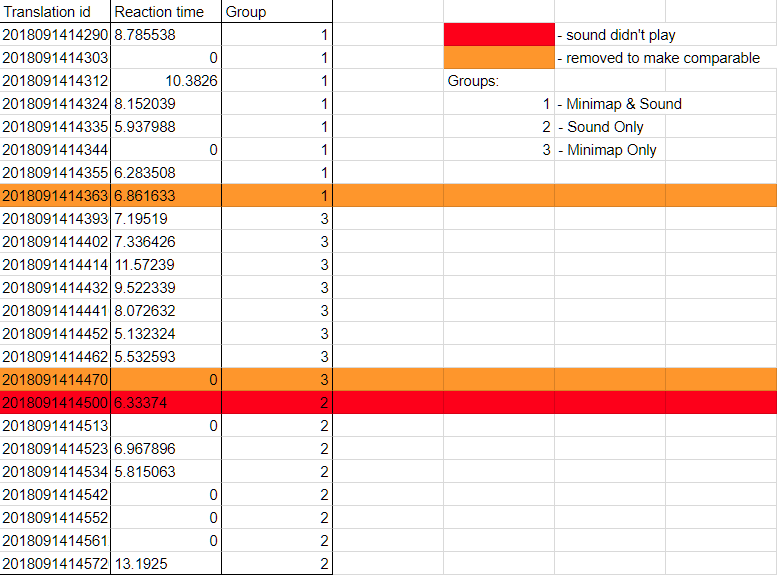
\includegraphics[width=0.7\linewidth]{figures/final_study_data_example}
	\caption{Data collected for a participant}
	\label{fig:finalstudydataexample}
\end{figure}
\end{comment}

When asked to rate different awareness presentations with an integer score from the most (1) to the least (3) useful, participants gave the feedback, shown in Fig. \ref{fig:finalstudyawarenesspresentationuserpreference}. They were allowed to give the same rating to different presentations (i.e. some participants ranked \textit{Minimap and Sound} and \textit{Sound Only} presentations with the same score \textemdash 1).

\begin{figure}
	\centering
	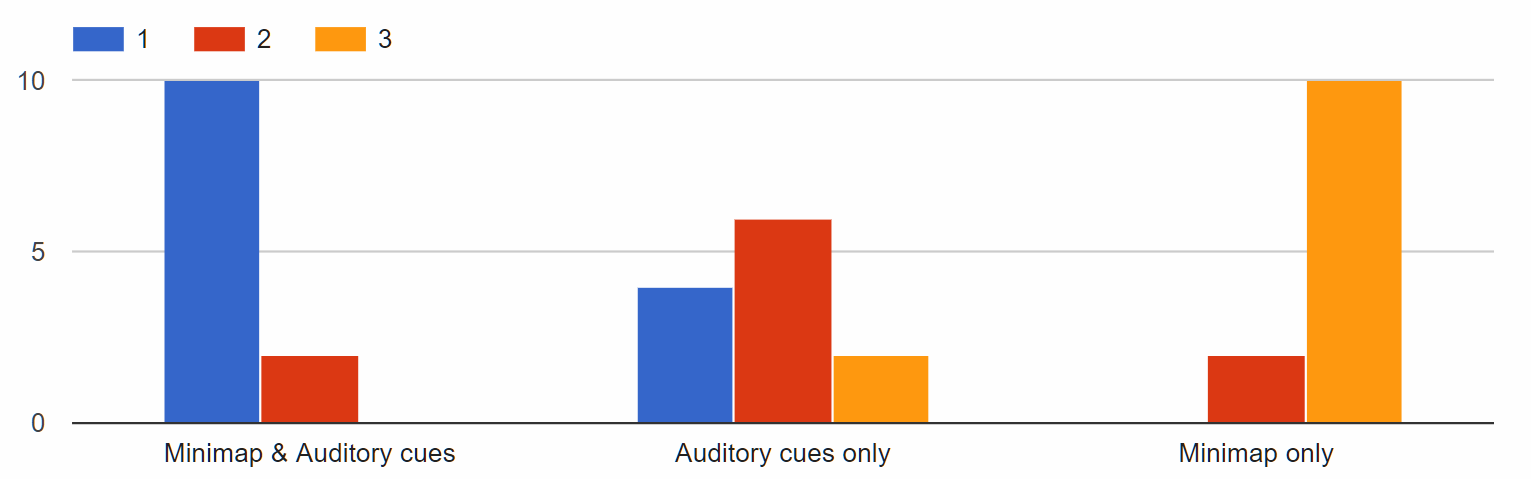
\includegraphics[width=0.7\linewidth]{figures/final_study_awareness_presentation_user_preference}
	\caption{Participants' preference of the awareness presentation}
	\label{fig:finalstudyawarenesspresentationuserpreference}
\end{figure}

Most participants managed to trace the first 3-4 shapes, only one was able to finish 6.

\paragraph{Discussion}
The visual analysis (Fig. \ref{fig:histograms_combined}, \ref{fig:distributions_freqReaction0}) shows that approx. $1/4$th of all the translations were not caught: 11 from Group 1, 19 from Group 2, and 26 from Group 3. % TODO: label multiple times defined?

Side-by-side distributions clearly indicate that Groups 1 and 2 took less time for participants to catch them (see the violin diagram in Fig \ref{fig:distributions_violin}). Generally, the distribution of the first two groups suggests their relative similarity. The fact that the \textit{Sound Only} group has the smallest reaction times could possibly be an error and the result of a building simply being in the participant's sight. The elongated top-handle of the distribution for the \textit{Sound Only} group could indicate that it was harder to catch the building after noticing it for the first time, which also correlates with the observations of the users during the experiment.

I observed that it was mostly due to the building or the minimap being in the participants' sight that they were able to spot the moving building in the \textit{Minimap Only} group. By contrast, in case of the groups that relied on the audio feedback, participants were always informed of translations happening, even if they had difficulties exactly locating it (i.e. in the \textit{Sound Only} group).

% TODO: about how the performance should also be judged by how focused the participants were on their main task 
% + figures of some of the voxel drawings (side-by-sides of the same shape to prove the point).

% TODO: None of the participants reported annoyence with the auditory cues, even though it was expected.

The results of the analysis and participant-feedback suggest that the additional audio feedback help users to improve their awareness of the workspace. The best best awareness presentation was the \textit{Minimap and Sound} group, followed by \textit{Sound Only} and \textit{Minimap Only}.

Statistical summary for each group can be found in Table \ref{tab:final_study_stats}.

\begin{figure}
	\centering
	
%	\subfloat[Combined histogram]{\label{fig:histograms_combined}\includegraphics[scale=.15]{D:/Documents/studies/ss18/Thesis/Studies/WorkspaceAwareness/RplotHistogram.png}}
	
	\begin{comment}
		\subfloat[Group 1]{\label{fig:distributions_g1}\includegraphics[scale=.15]{D:/Documents/studies/ss18/Thesis/Studies/WorkspaceAwareness/RplotHistogramGroup1.png}}
	
		\par \smallskip
		\subfloat[Group 2]{\label{fig:histograms_g2}\includegraphics[scale=.15]{D:/Documents/studies/ss18/Thesis/Studies/WorkspaceAwareness/RplotHistogramGroup2.png}}
		
		\subfloat[Group 3]{\label{fig:histograms_g3}\includegraphics[scale=.15]{D:/Documents/studies/ss18/Thesis/Studies/WorkspaceAwareness/RplotHistorgramGroup3.png}}
	\end{comment}
	
	\subfloat[Caught and missed translations]{\label{fig:distributions_freqReaction0}\includegraphics[width=0.7\linewidth]{D:/Documents/studies/ss18/Thesis/Studies/WorkspaceAwareness/TotalTranslations_CaughtUncaught_per_Group.png}}
	
	\par \smallskip
	%TODO: distribution in Google Sheets for aesthetics?
	\subfloat[Reaction time distribution per group, excluding uncaught buildings]{\label{fig:distributions_violin}\includegraphics[width=0.7\linewidth]{D:/Documents/studies/ss18/Thesis/Studies/WorkspaceAwareness/RplotViolinNon0}} % TODO: label multiple times defined? Like, meaning, in the same figure?
	
	\caption{Data distributions}
	\label{fig:histograms}
\end{figure}

\begin{table}[h]
	\caption{Statistical summary}
	\label{tab:final_study_stats}
	
	\begin{tabularx}{\linewidth}{|X|X|X|X|}
		\hline
		& \textbf{Group 1: Minimap and Sound} & \textbf{Group 2: Sound Only} & \textbf{Group 3: Minimap Only} \\ \hline
		\textbf{Mean (sec.)}  & 4.662725                            & 4.700911                     & 6.61726                        \\ \hline
		\textbf{St. dev. (sec.)}  & 2.266442                            & 2.483499                     & 2.73528                        \\ \hline
		\textbf{Range (sec.)} & {[}1.865601, 11.195500{]}           & {[}1.567505, 13.192500{]}    & {[}1.890381, 14.635010{]}      \\ \hline
		\textbf{Num. caught}  & 73                                  & 65                           & 58                             \\ \hline
	\end{tabularx}
\end{table}

\paragraph{Issues and shortcomings} \hfill

\textit{Data collection} Due to an issue with the implementation, sound wouldn't play occasionally for the first translation in the \textit{Sound Only}, \textit{Minimap and Sound}, or both groups. The entries where the sound did not play were removed from the dataset prior to its analysis (marked red in Table \ref{tab:finalstudy_datacollected}). Additionally, to make group observations comparable, in every group, where the sound did play on the first translation, or, like in case with the \textit{Minimap Only} group, the sound was never supposed to play, the last data entry for the group was removed (marked orange in Table \ref{tab:finalstudy_datacollected}). This way, experiment went from 8 observations per group for each participant to 7.

\textit{Motion sickness} The implementation of the voxel drawing system was not aimed at maximizing performance, as the result the frame rate dropped to approx. 70 FPS. One participants indicated feeling dizzy during one of such occurrences.

\textit{Minimap} Some users indicated that the minimap tool was not convenient, as they had to take of attention of their main task to attend to it. Different setups were tested for the mimap presentation during development: minimap attached to the \gls{hmd}, 4 minimaps placed above the participant (Fig. \ref{fig:finalstudyminimaparound}), and the hand-held minimap. While this will most likely be the case in any implementation, a possible solution would be to see the effects of having the minimap attached to the users head in a non-obstructive way.

\textit{Controls} Some users indicated that the controller mappings chosen for the final study were not convenient (Appendix \ref{app:finalstudy_controls}). Specifically, the fact that the main function of the 3D brush controller was mapped to the trigger, but for the minimap controller it was mapped to the touchpad. The controls were chosen this way, because drawing with your thumb constantly on the touchpad did not seem convenient, while the laser pointer's capabilities map perfectly to the two input modes for of a touchpad: the touch and press. The pressure sensitivity of the trigger does not provide such a clear separation between the press levels. This ambiguity of the mapping choice indicates that physical ergonomics factors also deserves an investigation in the current setup.

\begin{figure}[b]
	\centering
	\subfloat{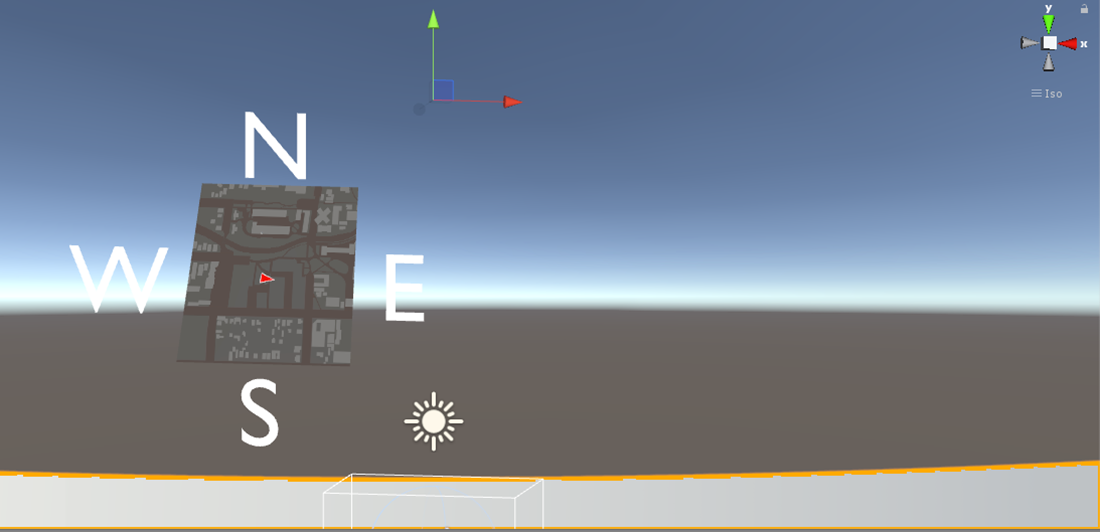
\includegraphics[width=0.7\linewidth]{figures/finalstudy_minimap_around1}}
	\par
	\subfloat{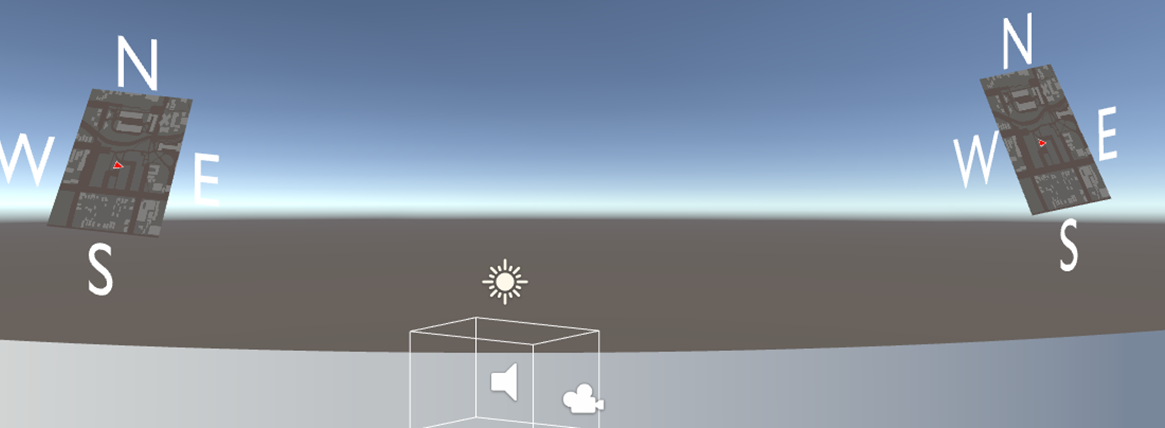
\includegraphics[width=0.7\linewidth]{figures/finalstudy_minimap_around2}}
	\caption{Minimap surrounding the participant}
	\label{fig:finalstudyminimaparound}
\end{figure}